\begin{frame}
\frametitle{What we want to introduce}
\begin{itemize}
\item Importance of search strategy, constraints alone are not enough
\item Two schools of thought
  \begin{itemize}
  \item Black-box solver, solver decides by itself
  \item Human control over process
  \end{itemize}
  
\item Dynamic variable ordering exploits information from propagation
\item Variable and value choice
\item Hard to find strategy which works all the time
%\item \texttt{int\_search} annotation, simple search abstraction
%  \item \texttt{seq\_search} and \texttt{priority\_search}, add flexibility
\item Different way of improving stability of search routine
\end{itemize}
\end{frame}

\begin{frame}
\frametitle{Example Problem}
\begin{itemize}
\item N-Queens puzzle
\item Rather weak constraint propagation
\item Many solutions, limited number of symmetries
\item Easy to scale problem size
\end{itemize}
\end{frame}

As example for the different techniques we use the N-Queens puzzle, a standard problem in Artificial Intelligence and Constraint Programming. The model we use has rather weak constraint propagation, there is not that much information that is deduced from the constraints, so that we rely more on search in solving this problem. The puzzle has many solutions, indeed too many to easily enumerate beyond sizes 10 or 12, and only a limited number of symmetries. A big advantage is that we can easily scale the problem size to create a number of related problem instances, which helps us to understand problems of stability of the methods considered.

\section{Problem}

Let's look at the problem in a bit more detail.

\begin{frame}
\frametitle{Problem Definition}
\begin{block}{8-Queens}
Place 8 queens on an $8\times 8$ chessboard so that no queen attacks another. A queen attacks all cells in horizontal, vertical and diagonal direction. Generalizes to boards of size $N\times N$.
\end{block}
\only<presentation>{
\vfill
\only<2>{
\begin{tabular}{cc}
\includegraphics[width=3cm]{../nqueen/compact/frame45}
&
Solution for board size $8\times 8$
\end{tabular}
}
}
\end{frame}

\begin{figure}[h]
\caption{\label{nqueen:solution8} Solution for board size $8\times 8$}
\begin{center}
\includegraphics[width=4cm]{../nqueen/compact/frame45}
\end{center}
\end{figure}

The 8-Queens puzzle is the problem of placing eight queens on a chess board so that no queen attacks another. A queen attacks all cells in horizontal, vertical or diagonal direction. The original puzzle is for an $8\times 8$ chess board. Obviously, we can easily generalize this problem to an arbitary board size $N\times N$.

The diagram (Figure~\ref{nqueen:solution8}) shows a solution for the $8\times 8$ case, the queens are marked in red. It is easy to see that no queen attacks any other queen in this solution. 

\section{Program}
We will now discuss how to model and solve this problem with ECLiPSe.

\subsection{Model}

\begin{frame}
\frametitle{Basic Model}
\begin{itemize}
\item Cell based Model
\begin{itemize}
\item A 0/1 variable for each cell to say if it is occupied or not
\item Constraints on rows, columns and diagonals to enforce no-attack
\item $N^2$ variables, $6N-2$ constraints
\end{itemize}
\item Column (Row) based Model
\begin{itemize}
\item A 1..N variable for each column, stating position of queen in the column
\item Based on observation that each column must contain exactly one queen
\item $N$ variables, $N^2/2$ binary constraints
\end{itemize}
\end{itemize}
\end{frame}

There are basically two models for this problem, one based on cells, the other on columns (or rows).

In the first model we introduce 0/1 integer variables for all cells, they describe if a cell contains a queen or not. Linear constraints on the rows, columns and the diagonals enforce that there is at most one queen in each of them. We also have a constraint stating that we must place $N$ queens. This means that we have $N^2$ variables, and $N+N+2*(2N-1)+1 = 6N-1$ constraints.

The alternative to this model is a column (or row) based model, where we have a variable for each column (or row) of the board. This is based on the observation that each column must contain exactly one queen. If a column contains more than one queen, they would attack each other. A column can also not be empty. We need $N$ queens, and we have $N$ columns, each containing atmost one queen. By the {\em pigeon-hole principle} we know that there can be no empty columns, each must contain exactly one queen. The variable for a column then ranges over the values from 1 to $N$, and gives the position of the queen in the column.

This choice of model automatically handles the no-attack condition in the vertical direction, so we don't need a special constraint for this. In the horizontal direction we can express the no-attack condition by a binary disequality between any two column variables, i.e. the variables can not have the same values. But this means the variables must be pairwise different, and that is just the definition of the \texttt{alldifferent} constraint, which we already encountered in earlier examples. We can therefore express the no-attack condition in horizontal direction by a single \texttt{alldifferent} constraint between all variables.

This leaves us with the no-attack condition for the diagonals. They can also be expressed by disequalities, but we have to add an offset between the variables, which is based on their distance $j-i$. 

\begin{frame}
\frametitle{Model}
\[
\textrm{assign}\quad [X_1,X_2,...X_N]
\]
s.t.
\begin{align*}
\forall 1 \leq i \leq N:&\quad X_i \in 1..N\\
\forall 1 \leq i<j \leq N:&\quad X_i \neq X_j\\
\forall 1 \leq i<j \leq N:&\quad X_i +j\neq X_j+i\\
\forall 1 \leq i<j \leq N:&\quad X_i +i\neq X_j+j
\end{align*}
\end{frame}

We can write down our model in a concise mathematical form as a set of constraints and use this as the basis for our ECLiPSe program.


\section{Naive Search}

\begin{frame}
\frametitle{Nqueens Models}
\begin{itemize}
\item ECLiPSe \hyperlink{nqueens:eclipse}{\beamergotobutton{Show}}
\item MiniZinc \hyperlink{nqueens:minizinc}{\beamergotobutton{Show}}
\item NumberJack \hyperlink{nqueens:numberjack}{\beamergotobutton{Show}}
\item CPMpy \hyperlink{nqueens:cpmpy}{\beamergotobutton{Show}}
\item Choco-solver \hyperlink{nqueens:choco}{\beamergotobutton{Show}}
\end{itemize}
\end{frame}

\begin{frame}[fragile]
\frametitle{ECLiPSe N-Queens Model}
\label{nqueens:eclipse}
\tiny
\begin{verbatim}
:- lib(lists).
:- lib(ic).
:- lib(ic_search).

top:-
    queens(8,Board),
    search(Board, 0, input_order, indomain, complete).
    
queens(N, Board) :-
    length(Board, N),
    Board :: 1..N,
    ( fromto(Board, [Q1|Cols], Cols, []) do
        ( foreach(Q2, Cols), param(Q1), count(Dist,1,_) do
            noattack(Q1, Q2, Dist)
        )
    ).

noattack(Q1,Q2,Dist) :-
    Q2 #\= Q1,
    Q2 - Q1 #\= Dist,
    Q1 - Q2 #\= Dist.
\end{verbatim}
\hyperlink{nqueens:continue}{\beamergotobutton{Continue}}
\end{frame}


\begin{frame}[fragile]
  \frametitle{MiniZinc N-Queens Model}
  \label{nqueens:minizinc}
  \tiny
  \begin{semiverbatim}
int: n=8;
array[1..n] of var 1..n: queens;
constraint
    forall(i, j in 1..n where i < j) (
         queens[i] != queens[j] /\\
         queens[i] + i != queens[j] + j /\\
         queens[i] - i != queens[j] - j
    )
 ;
solve :: int\_search(
        queens,
        input\_order,
        indomain\_min)
        satisfy;
  \end{semiverbatim}
\hyperlink{nqueens:continue}{\beamergotobutton{Continue}}
\end{frame}

\begin{frame}[fragile]
\frametitle{NumberJack N-Queens Model}
\label{nqueens:numberjack}
\tiny
\begin{verbatim}
from Numberjack import *
 
def get_model(N):
    queens = VarArray(N, N)
    model = Model(
        AllDiff(queens),
        AllDiff([queens[i] + i for i in range(N)]),
        AllDiff([queens[i] - i for i in range(N)])
    )
    return queens, model
 
def solve(param):
    queens, model = get_model(param['N'])
    solver = model.load(param['solver'])
    solver.setHeuristic(param['heuristic'], param['value'])
    solver.setVerbosity(param['verbose'])
    solver.setTimeLimit(param['tcutoff'])
    solver.solve()
\end{verbatim}
\hyperlink{nqueens:continue}{\beamergotobutton{Continue}}
\end{frame}

\begin{frame}[fragile]
\frametitle{CPMpy N-Queens Model}
\label{nqueens:cpmpy}
\tiny
\begin{verbatim}
def nqueens_naive(n=8):
    queens = IntVar(1,n, shape=n)

    model = Model()
    for i in range(n):
        for j in range(i):
            model += [queens[i] != queens[j],
                  queens[i] + i != queens[j] + j,
                  queens[i] - i != queens[j] - j,
                  ]            
\end{verbatim}
\hyperlink{nqueens:continue}{\beamergotobutton{Continue}}
\end{frame}


\begin{frame}[fragile]
\frametitle{Choco-solver N-Queens Program}
\tiny
\label{nqueens:choco}
\begin{verbatim}
int n = 8;
Model model = new Model(n + "-queens problem");
IntVar[] vars = new IntVar[n];
for(int q = 0; q < n; q++){
    vars[q] = model.intVar("Q_"+q, 1, n);
}
for(int i  = 0; i < n-1; i++){
    for(int j = i + 1; j < n; j++){
        model.arithm(vars[i], "!=",vars[j]).post();
        model.arithm(vars[i], "!=", vars[j], "-", j - i).post();
        model.arithm(vars[i], "!=", vars[j], "+", j - i).post();
    }
}
Solution solution = model.getSolver().findSolution();
if(solution != null){
    System.out.println(solution.toString());
}
\end{verbatim}
\hyperlink{nqueens:continue}{\beamergotobutton{Continue}}
\end{frame}



When it comes to search, it does not matter which variant of the program we use. They create the same constraints, and assign the variables in the same order from $X_1$ to $X_N$. We will now use some visualization to see how the search routine finds its first solution.
 
\begin{frame}<presentation>
\frametitle{Default Strategy}
\label{nqueens:continue}
\only<beamer>{
\begin{textblock}{4}(10,1)
\only<1>{\includegraphics[width=3cm]{../nqueen/full/frame1}}
\only<2>{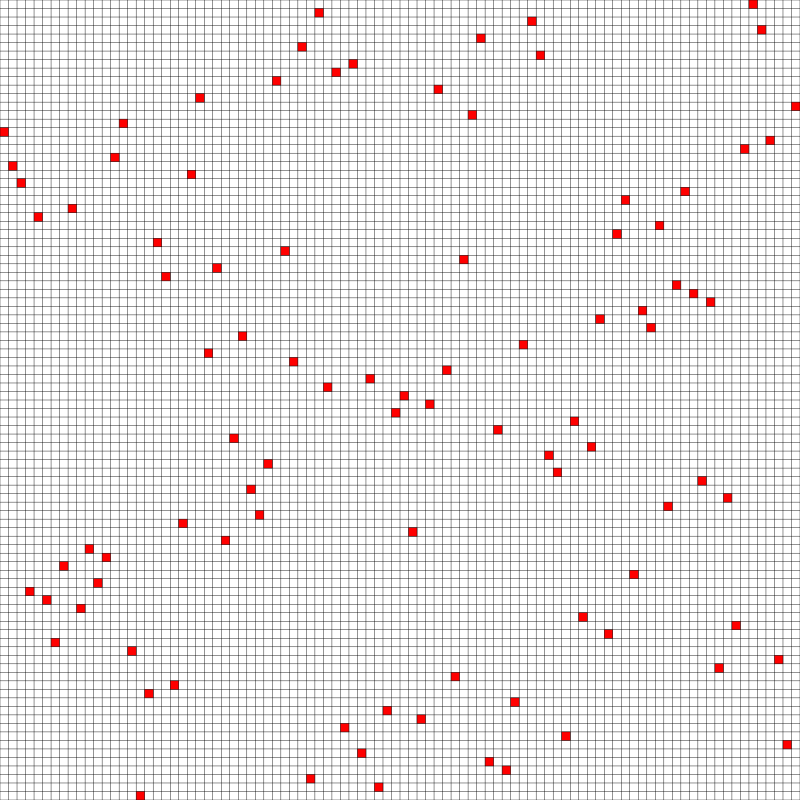
\includegraphics[width=3cm]{../nqueen/full/frame2}}
\only<3>{\includegraphics[width=3cm]{../nqueen/full/frame3}}
\only<4>{\includegraphics[width=3cm]{../nqueen/full/frame4}}
\only<5>{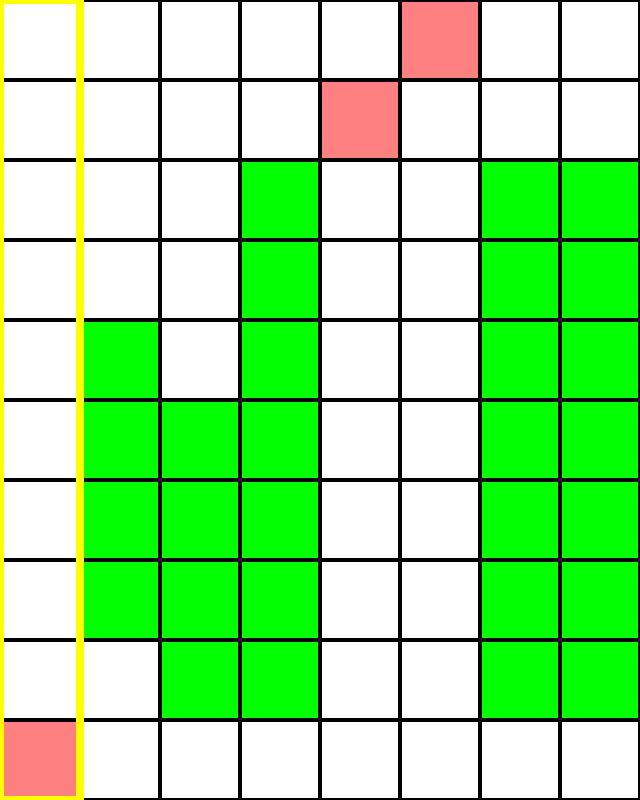
\includegraphics[width=3cm]{../nqueen/full/frame5}}
\only<6>{\includegraphics[width=3cm]{../nqueen/full/frame6}}
\only<7>{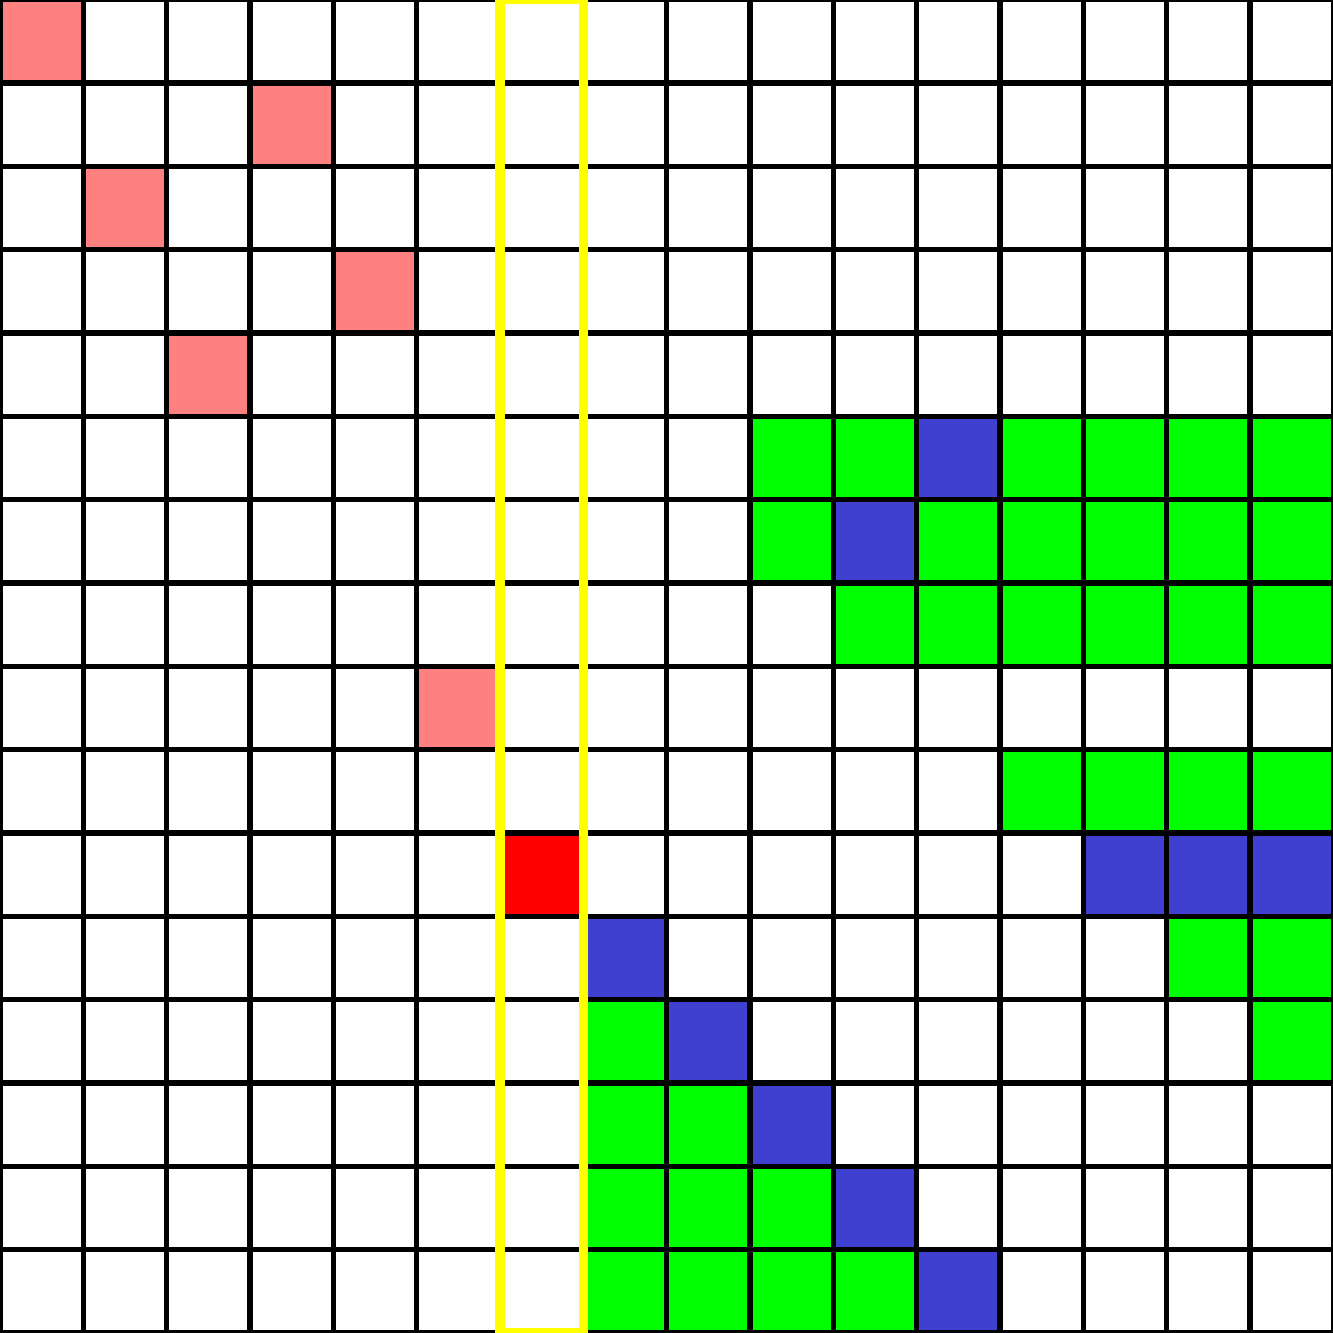
\includegraphics[width=3cm]{../nqueen/full/frame7}}
\only<8>{\includegraphics[width=3cm]{../nqueen/full/frame8}}
\only<9>{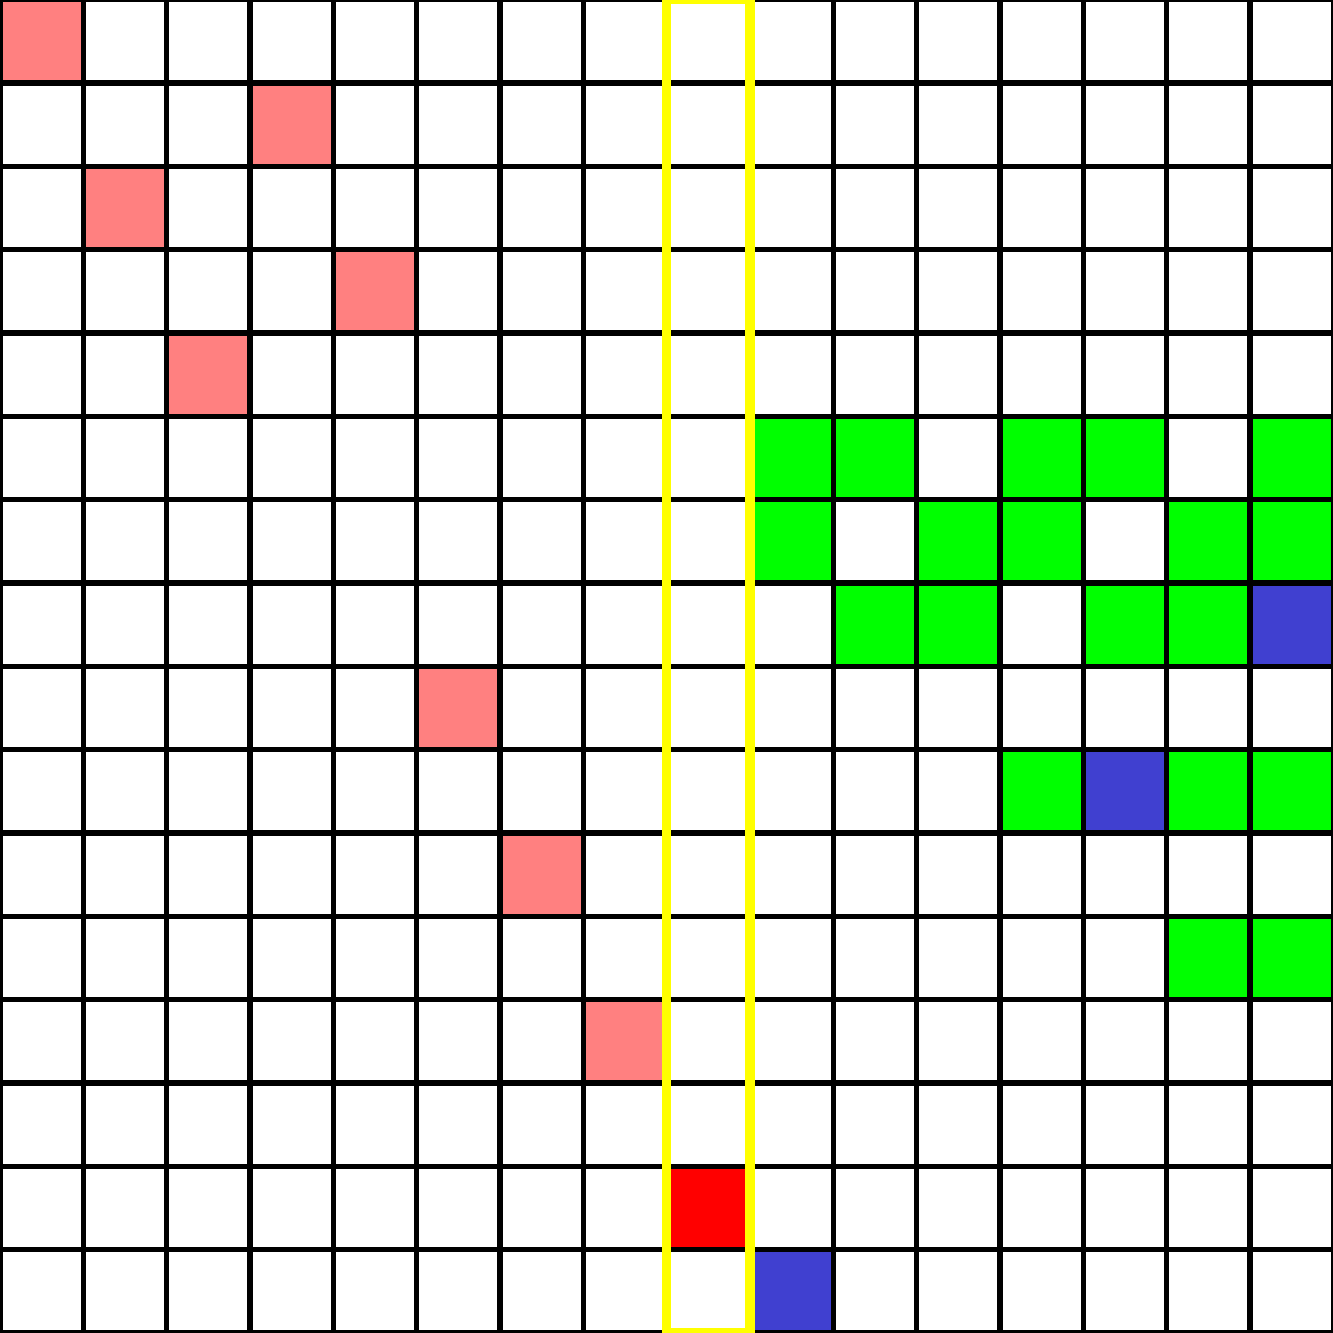
\includegraphics[width=3cm]{../nqueen/full/frame9}}
\only<10>{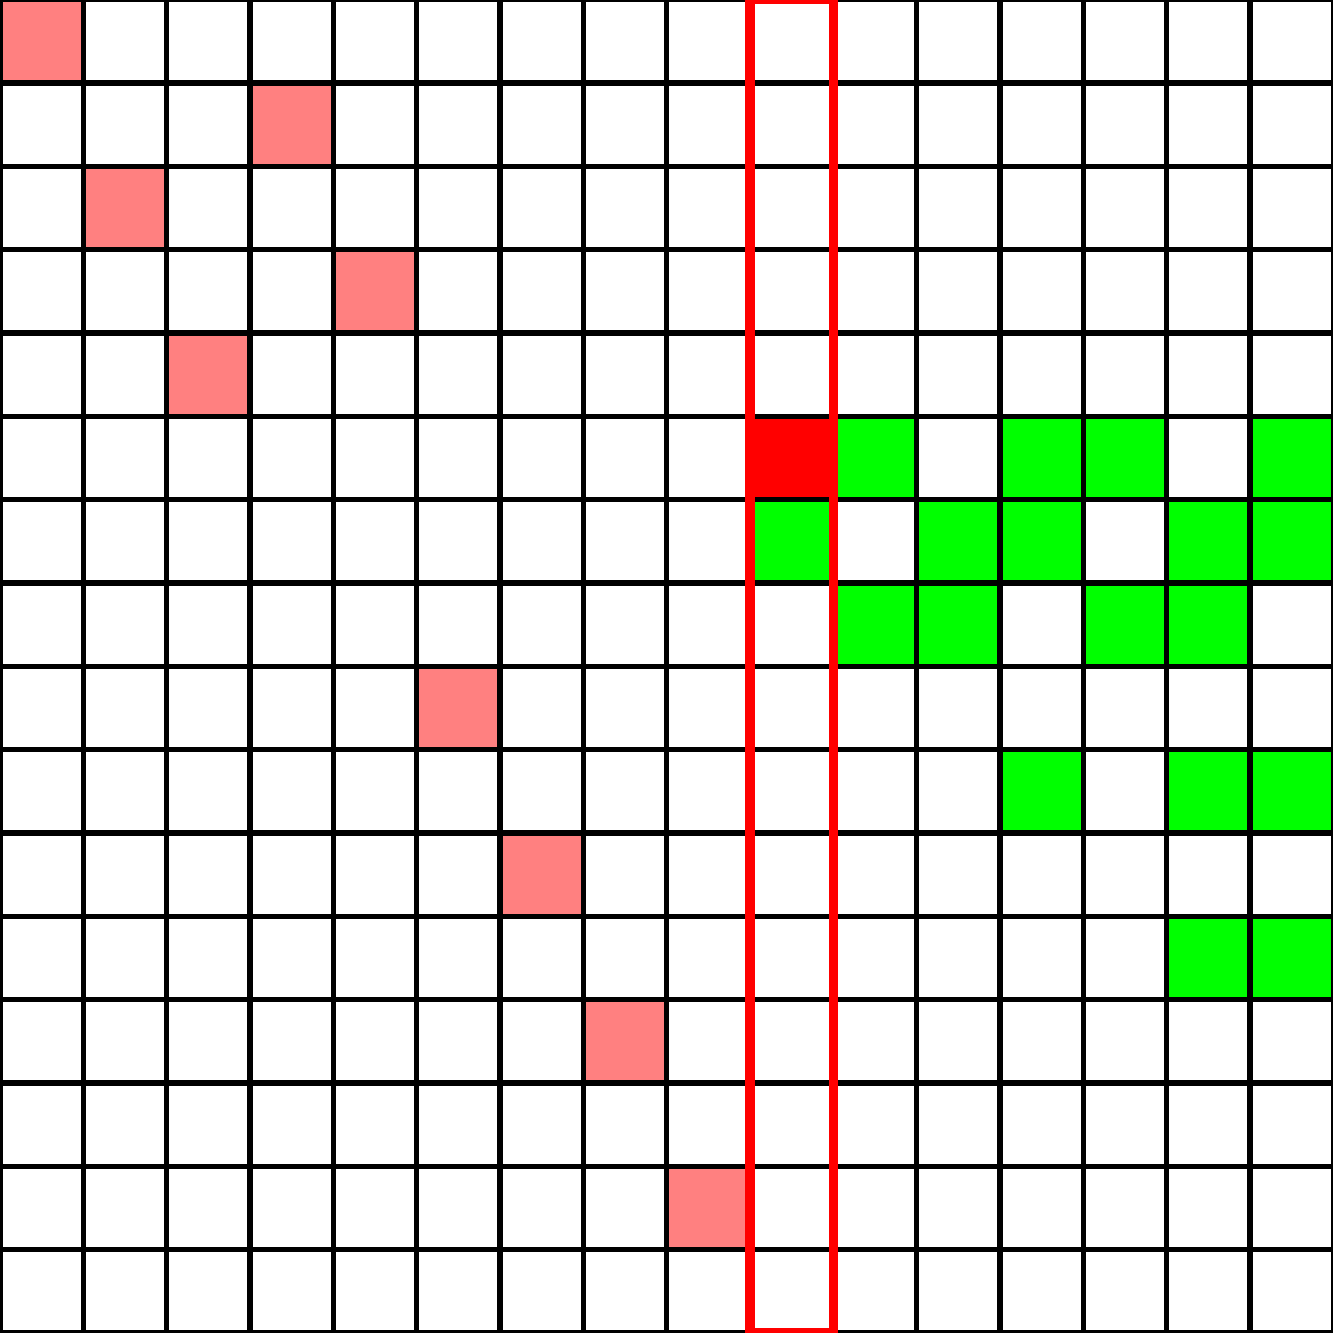
\includegraphics[width=3cm]{../nqueen/full/frame10}}
\only<11>{\includegraphics[width=3cm]{../nqueen/full/frame11}}
\only<12>{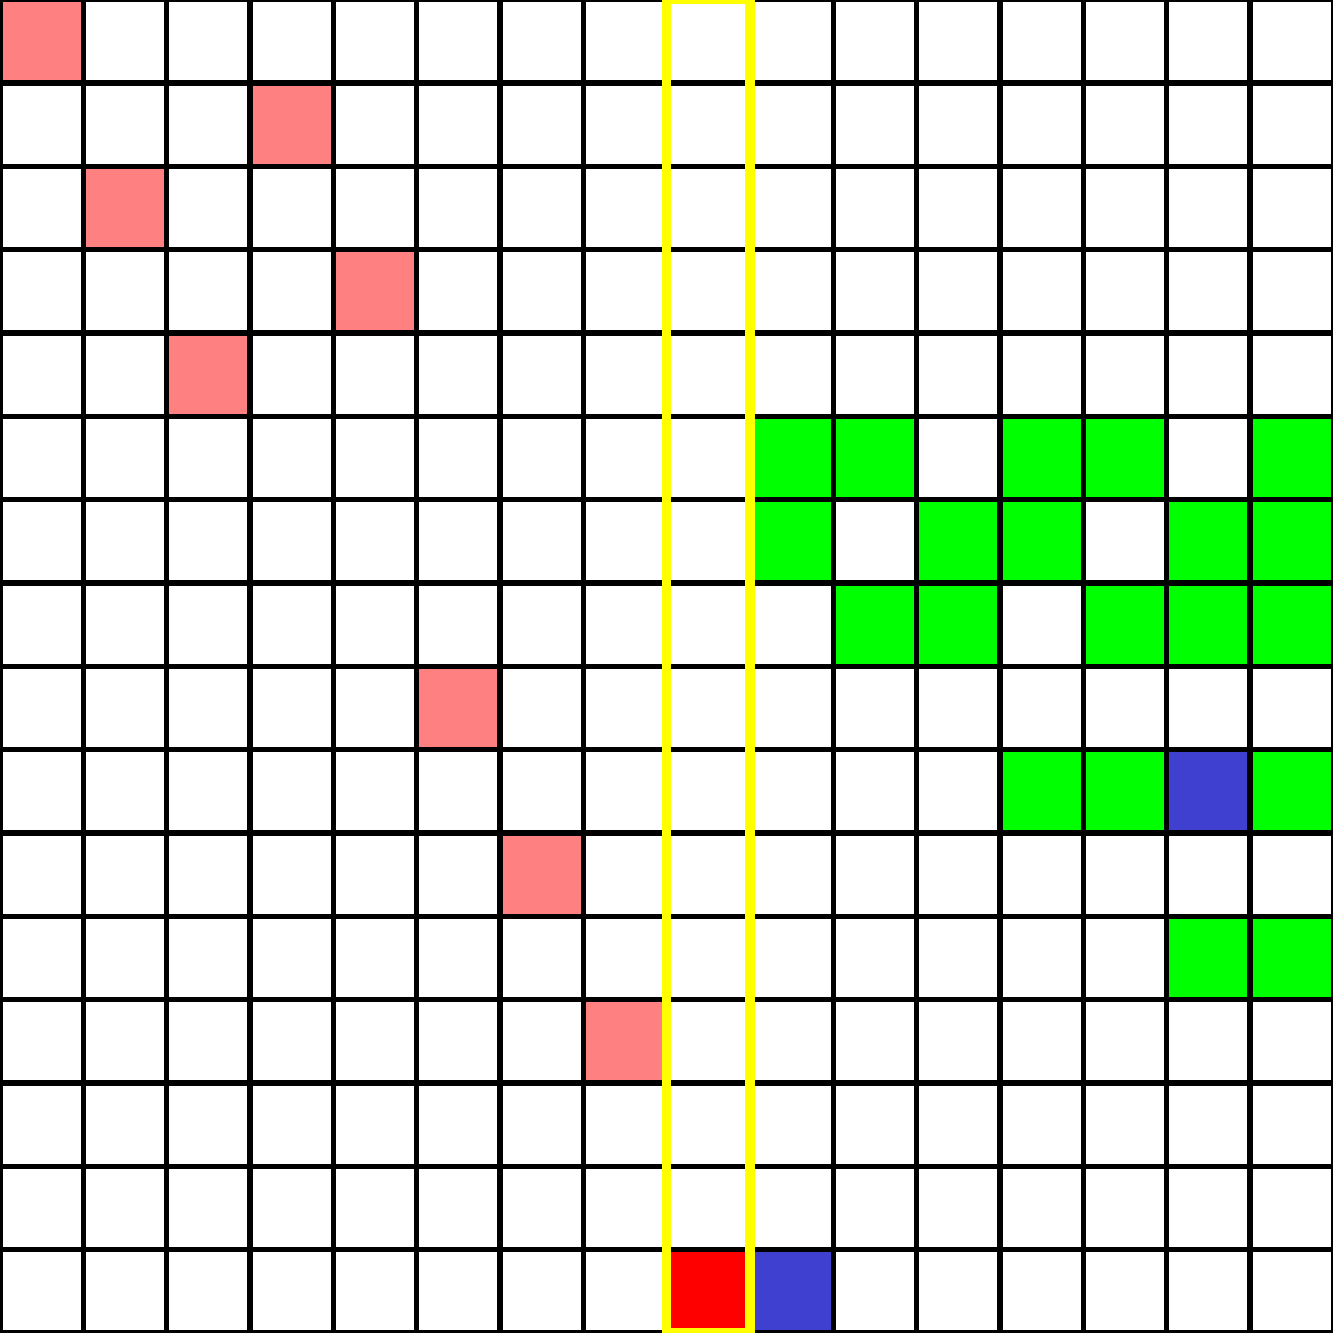
\includegraphics[width=3cm]{../nqueen/full/frame12}}
\only<13>{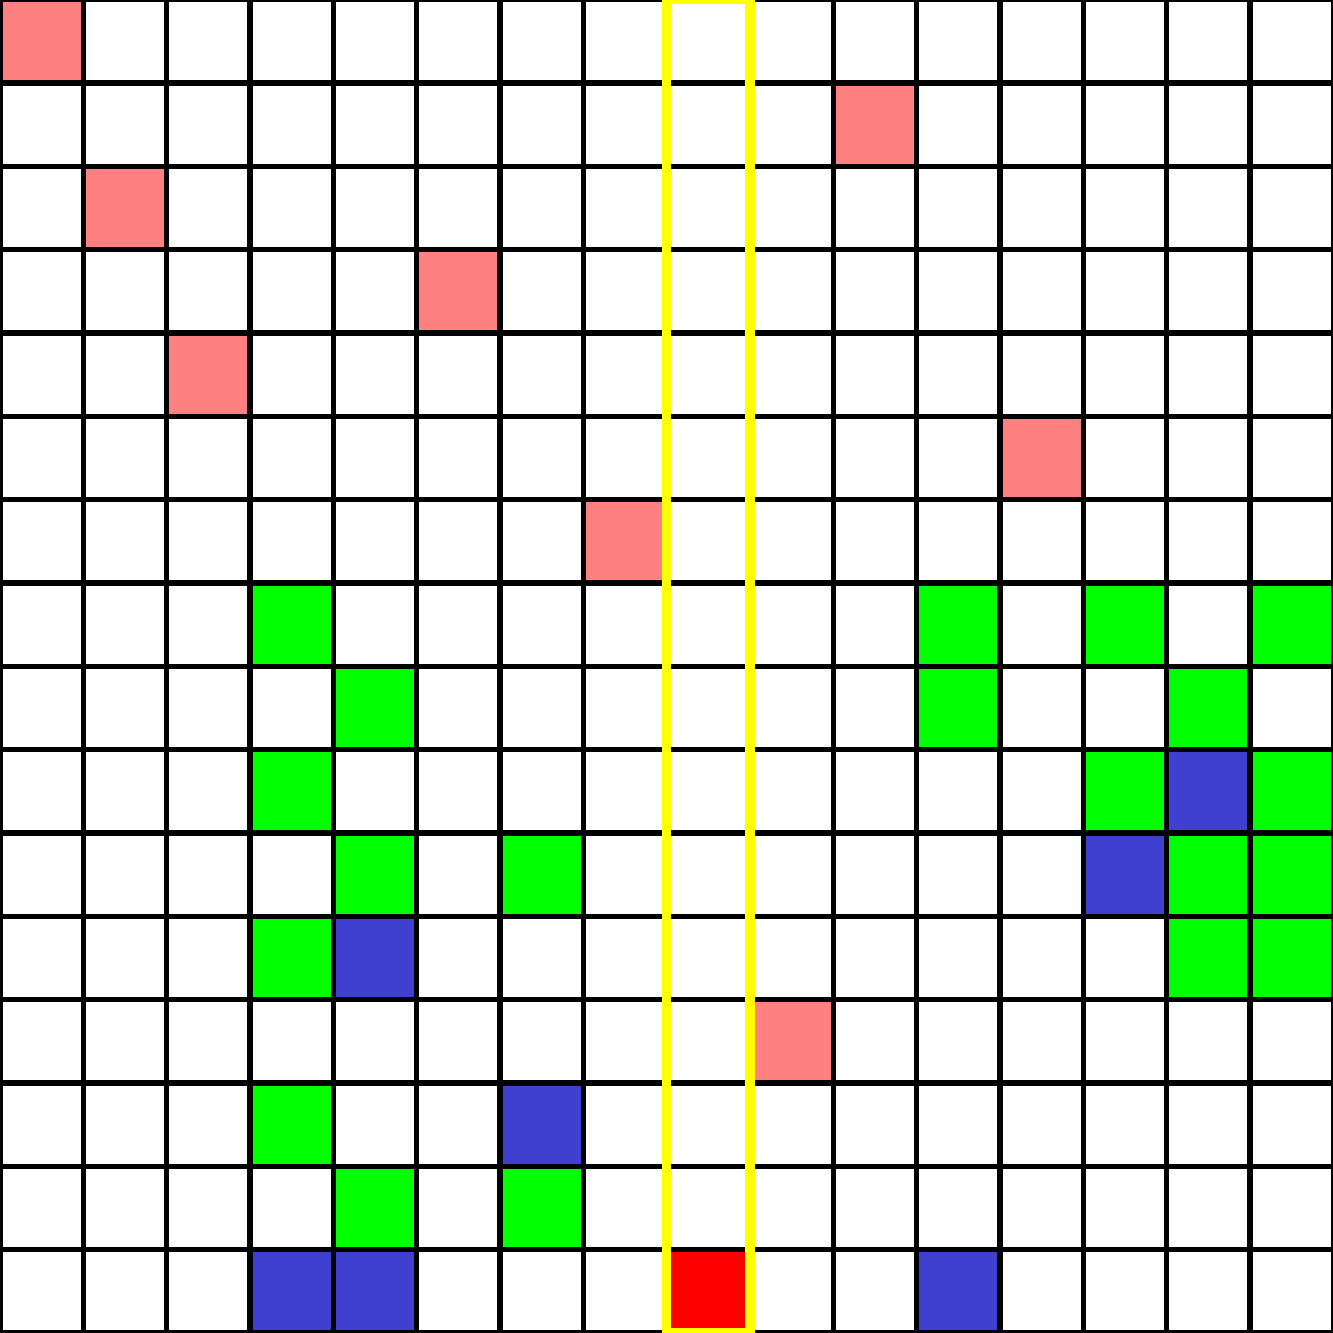
\includegraphics[width=3cm]{../nqueen/full/frame13}}
\only<14>{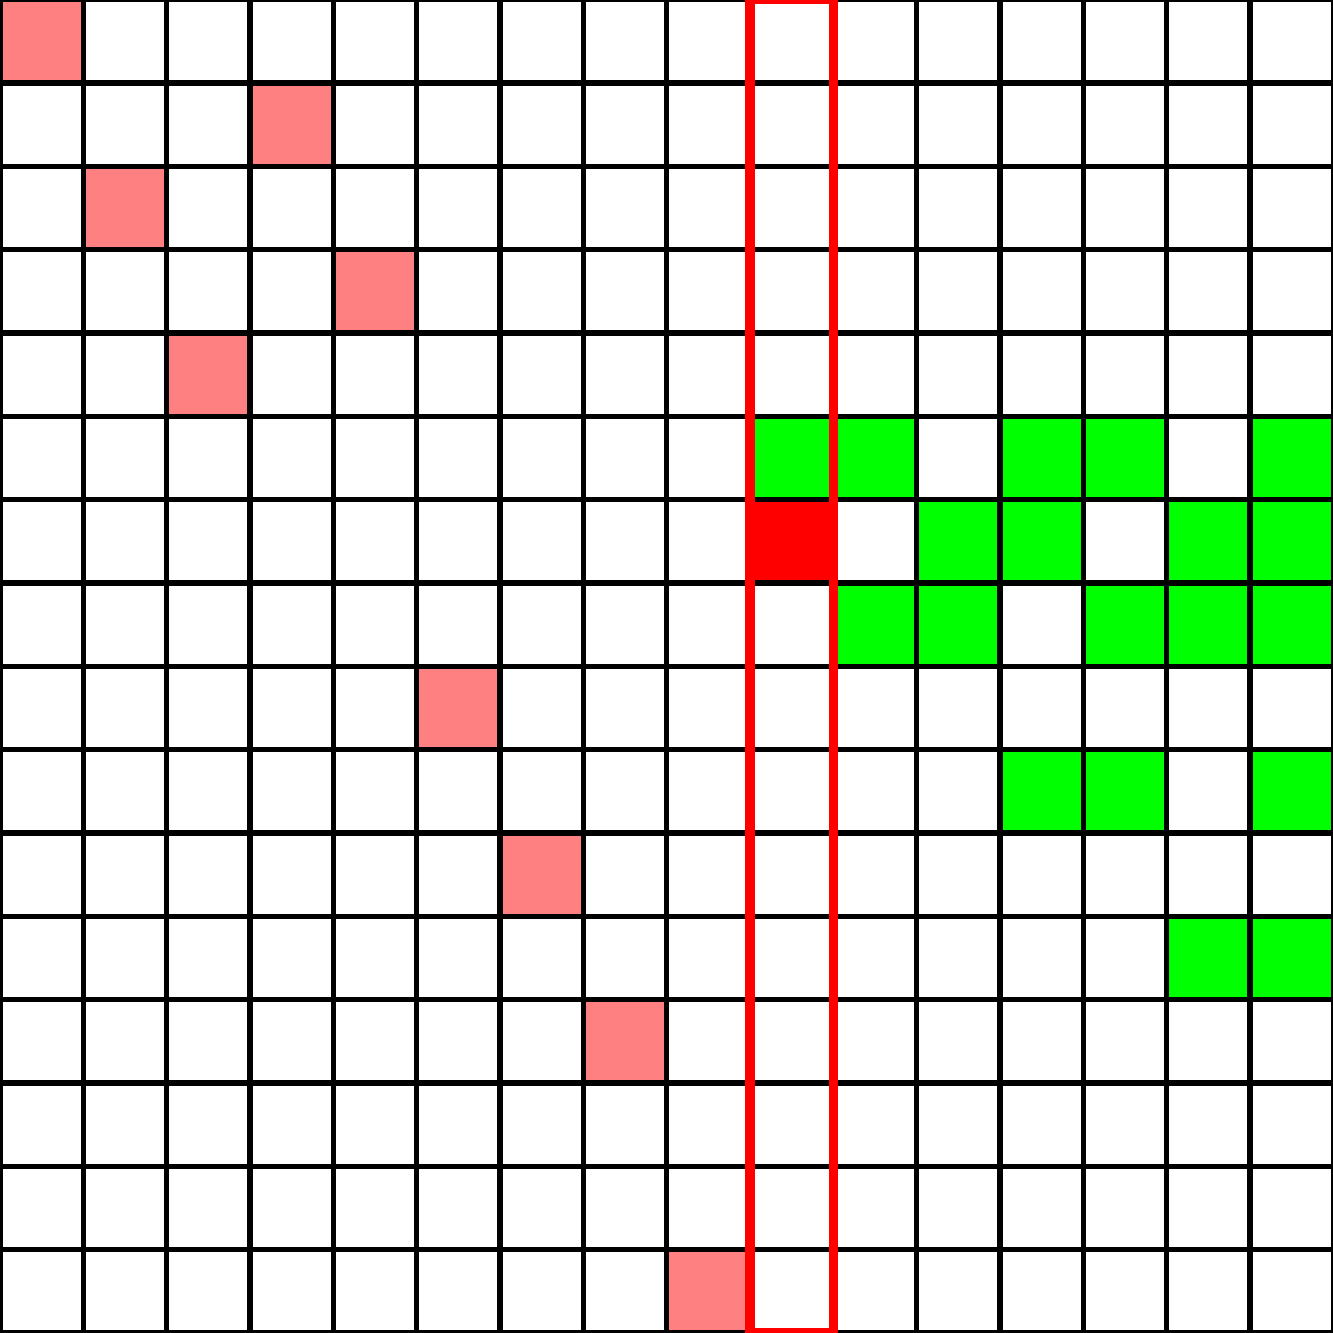
\includegraphics[width=3cm]{../nqueen/full/frame14}}
\only<15>{\includegraphics[width=3cm]{../nqueen/full/frame15}}
\only<16>{\includegraphics[width=3cm]{../nqueen/full/frame16}}
\only<17>{\includegraphics[width=3cm]{../nqueen/full/frame17}}
\only<18>{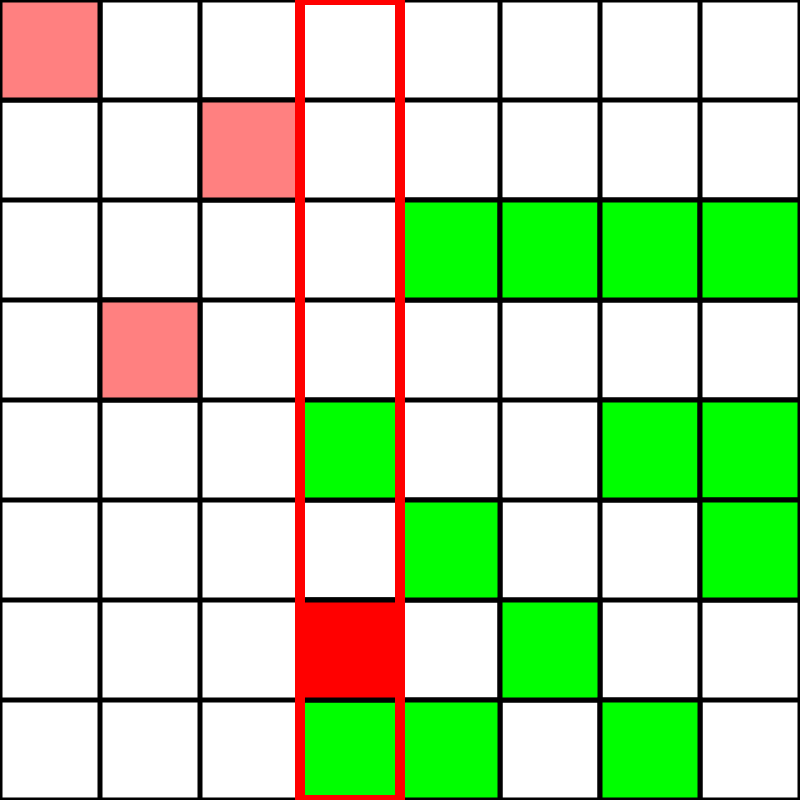
\includegraphics[width=3cm]{../nqueen/full/frame18}}
\only<19>{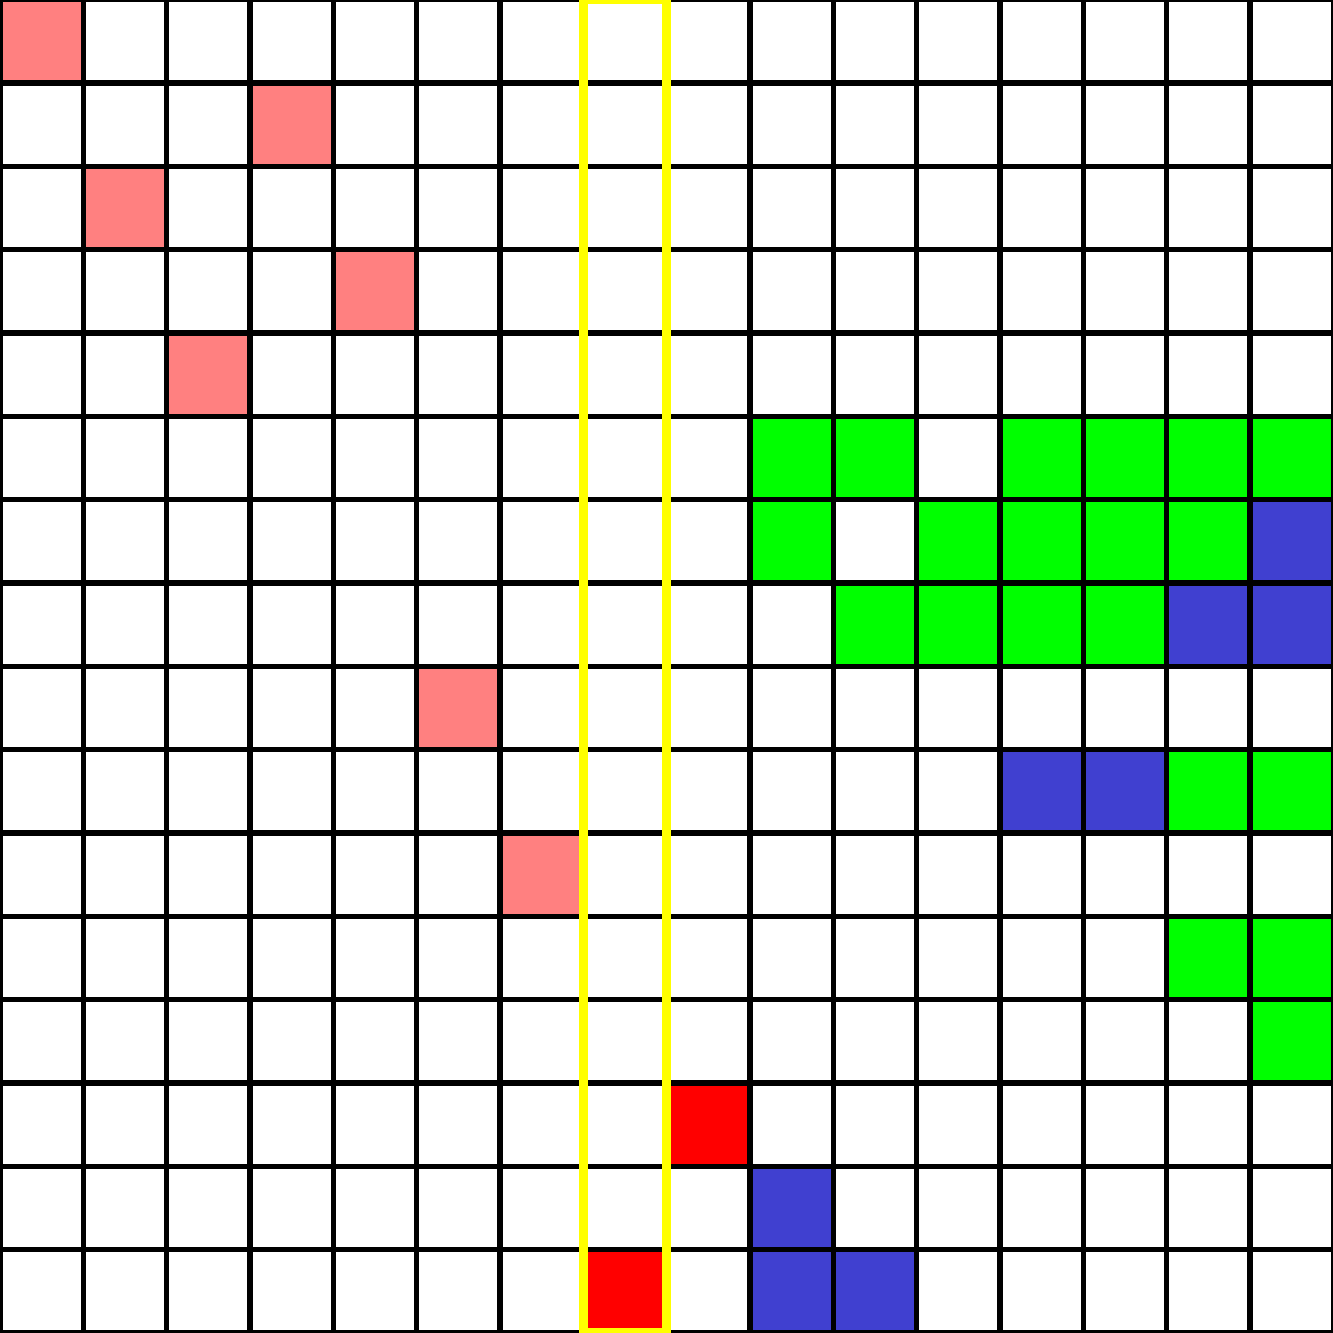
\includegraphics[width=3cm]{../nqueen/full/frame19}}
\only<20>{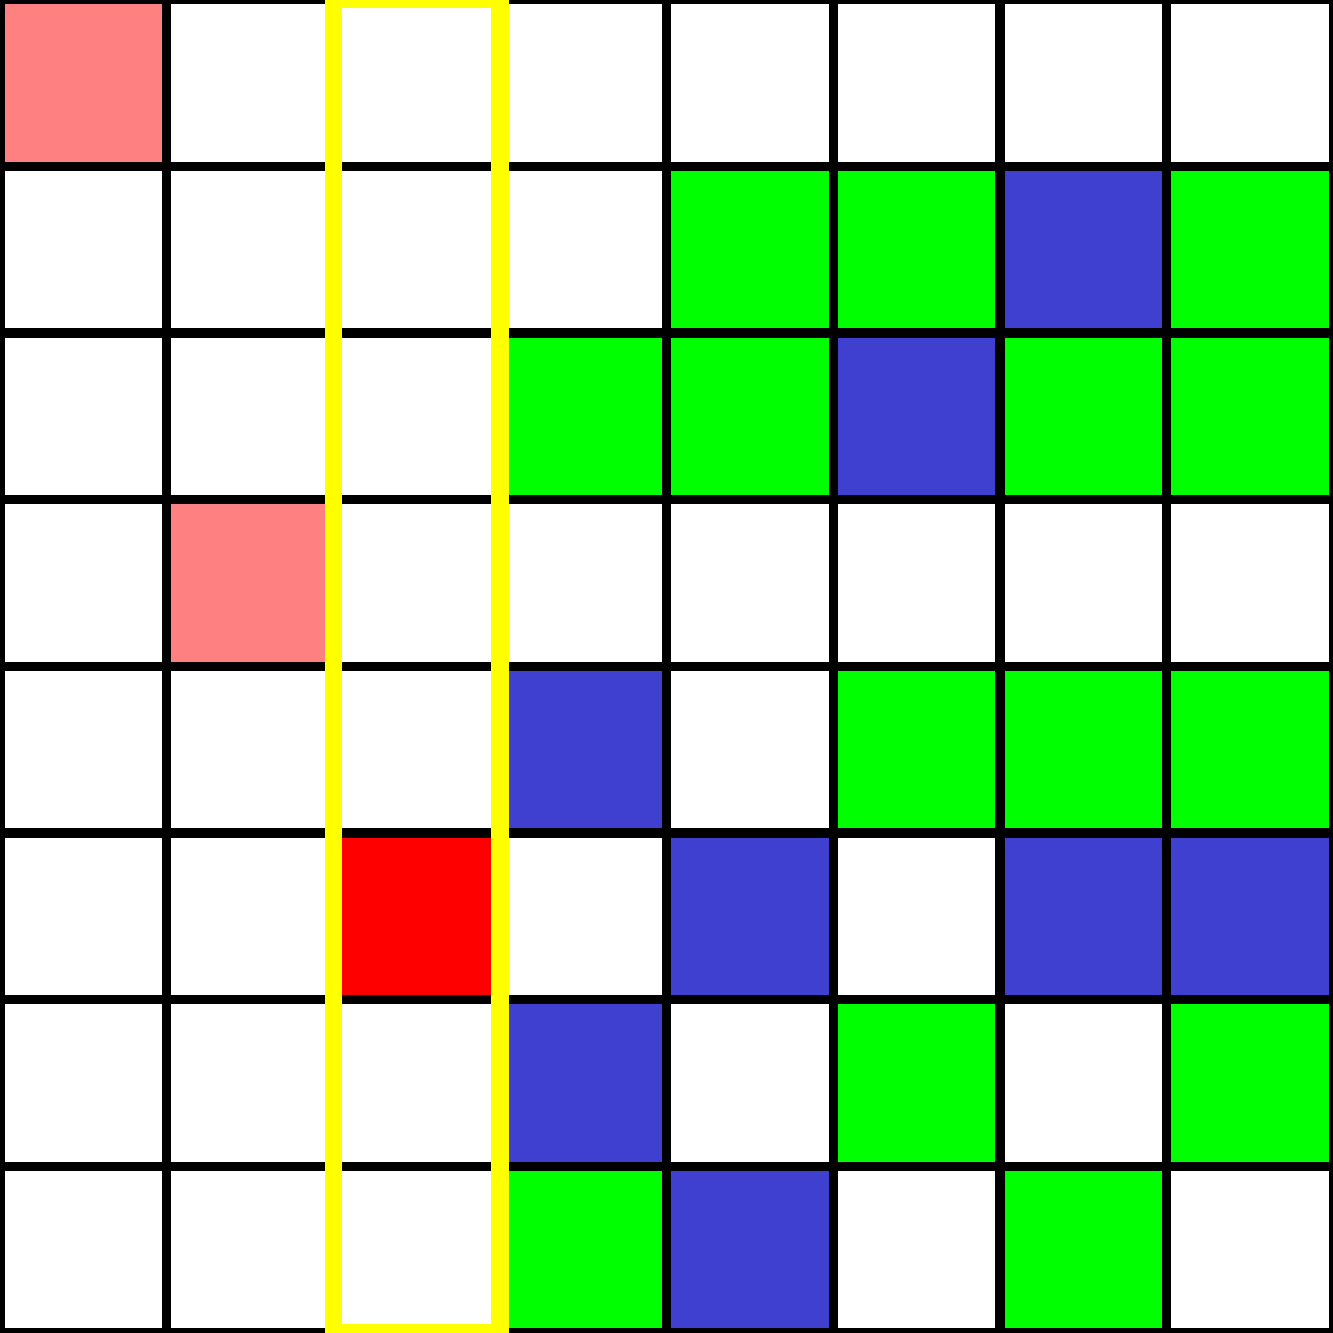
\includegraphics[width=3cm]{../nqueen/full/frame20}}
\only<21>{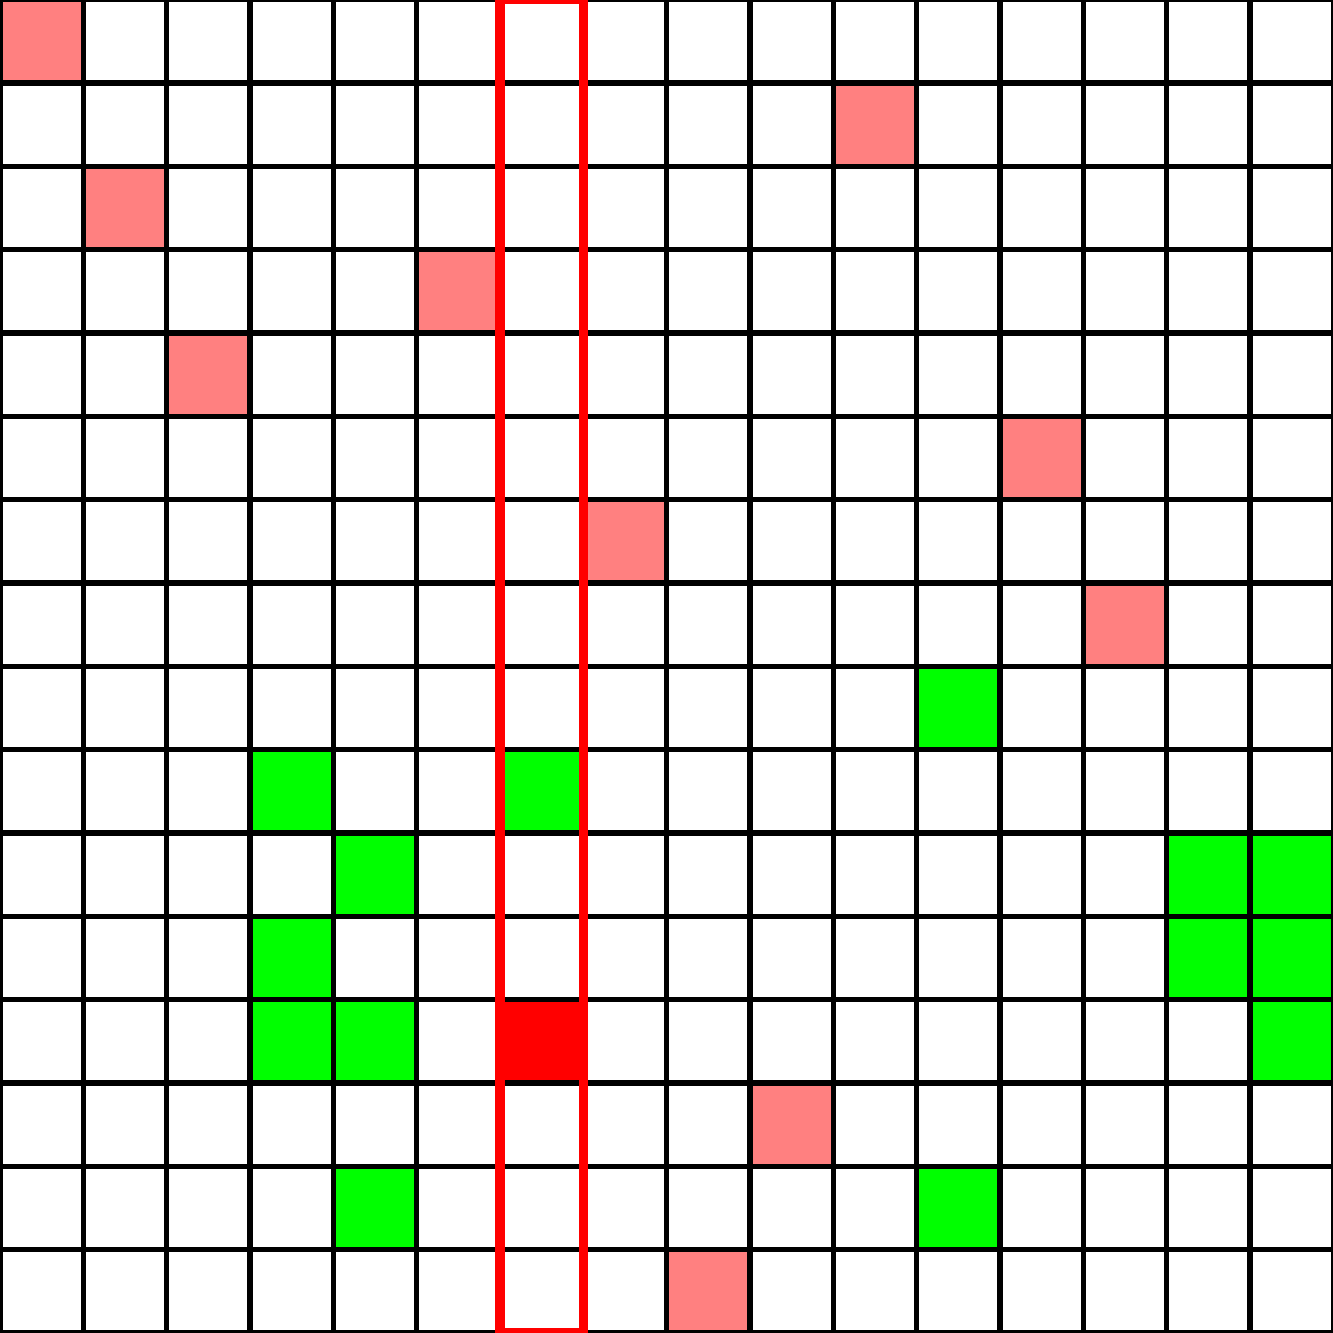
\includegraphics[width=3cm]{../nqueen/full/frame21}}
\only<22>{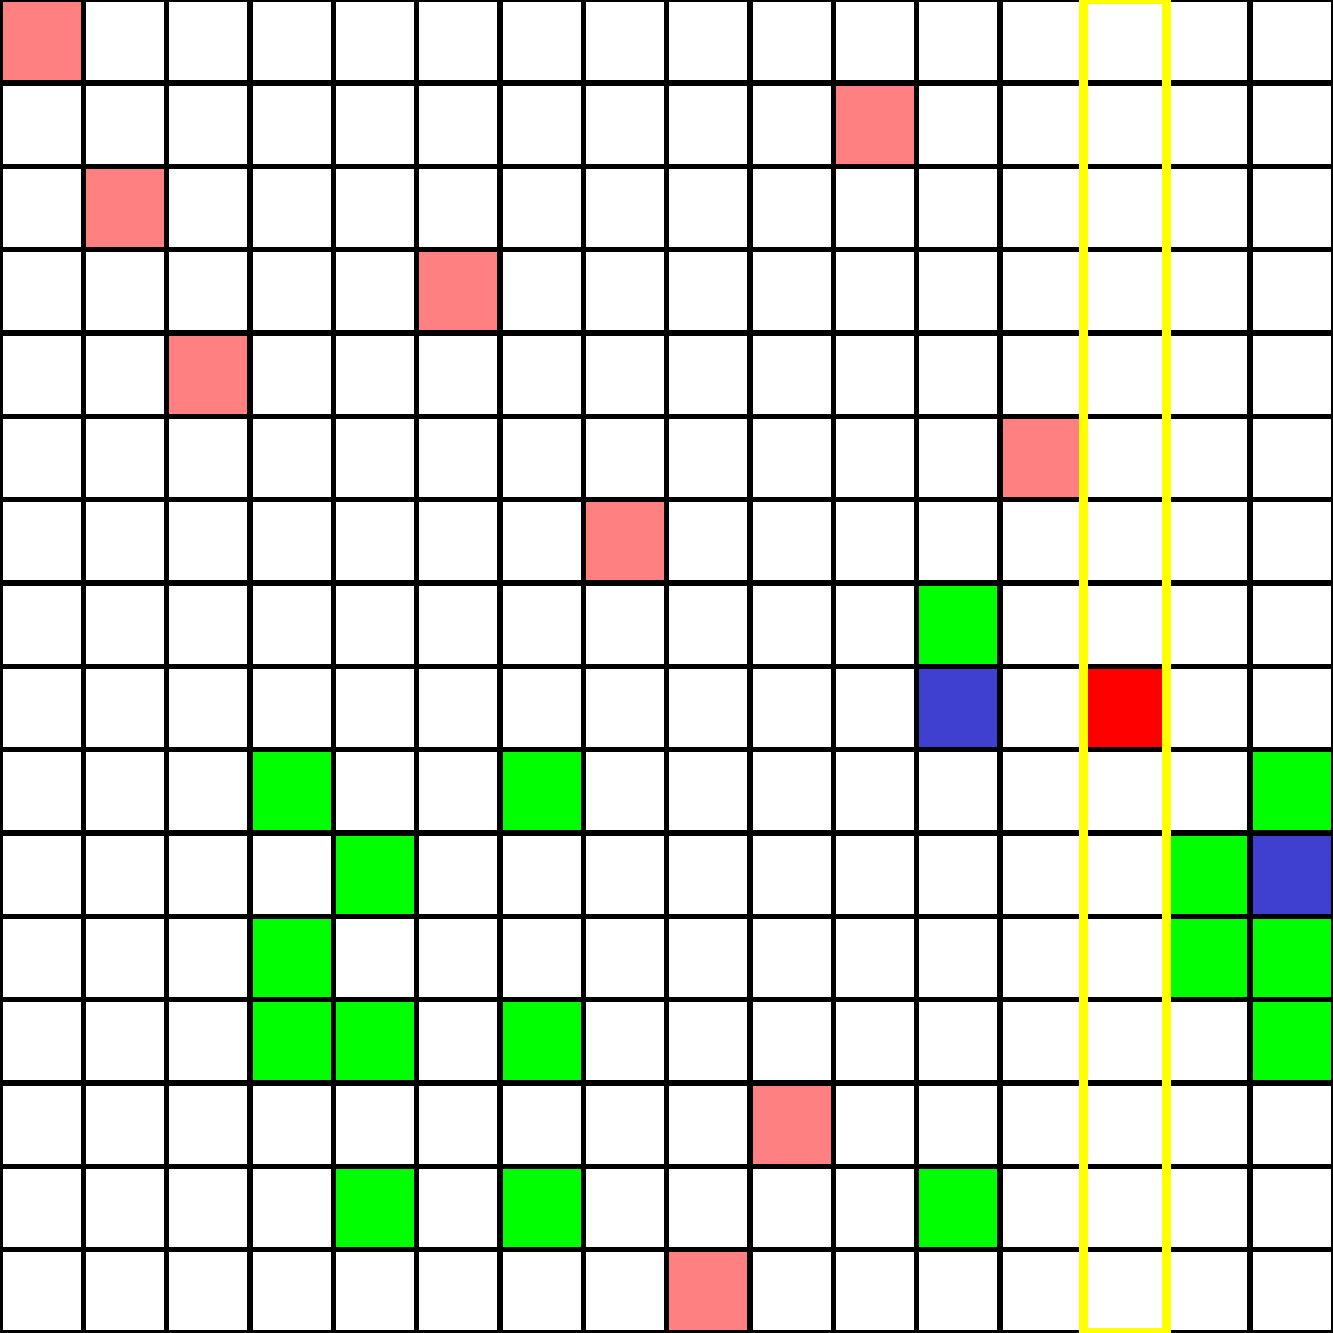
\includegraphics[width=3cm]{../nqueen/full/frame22}}
\only<23>{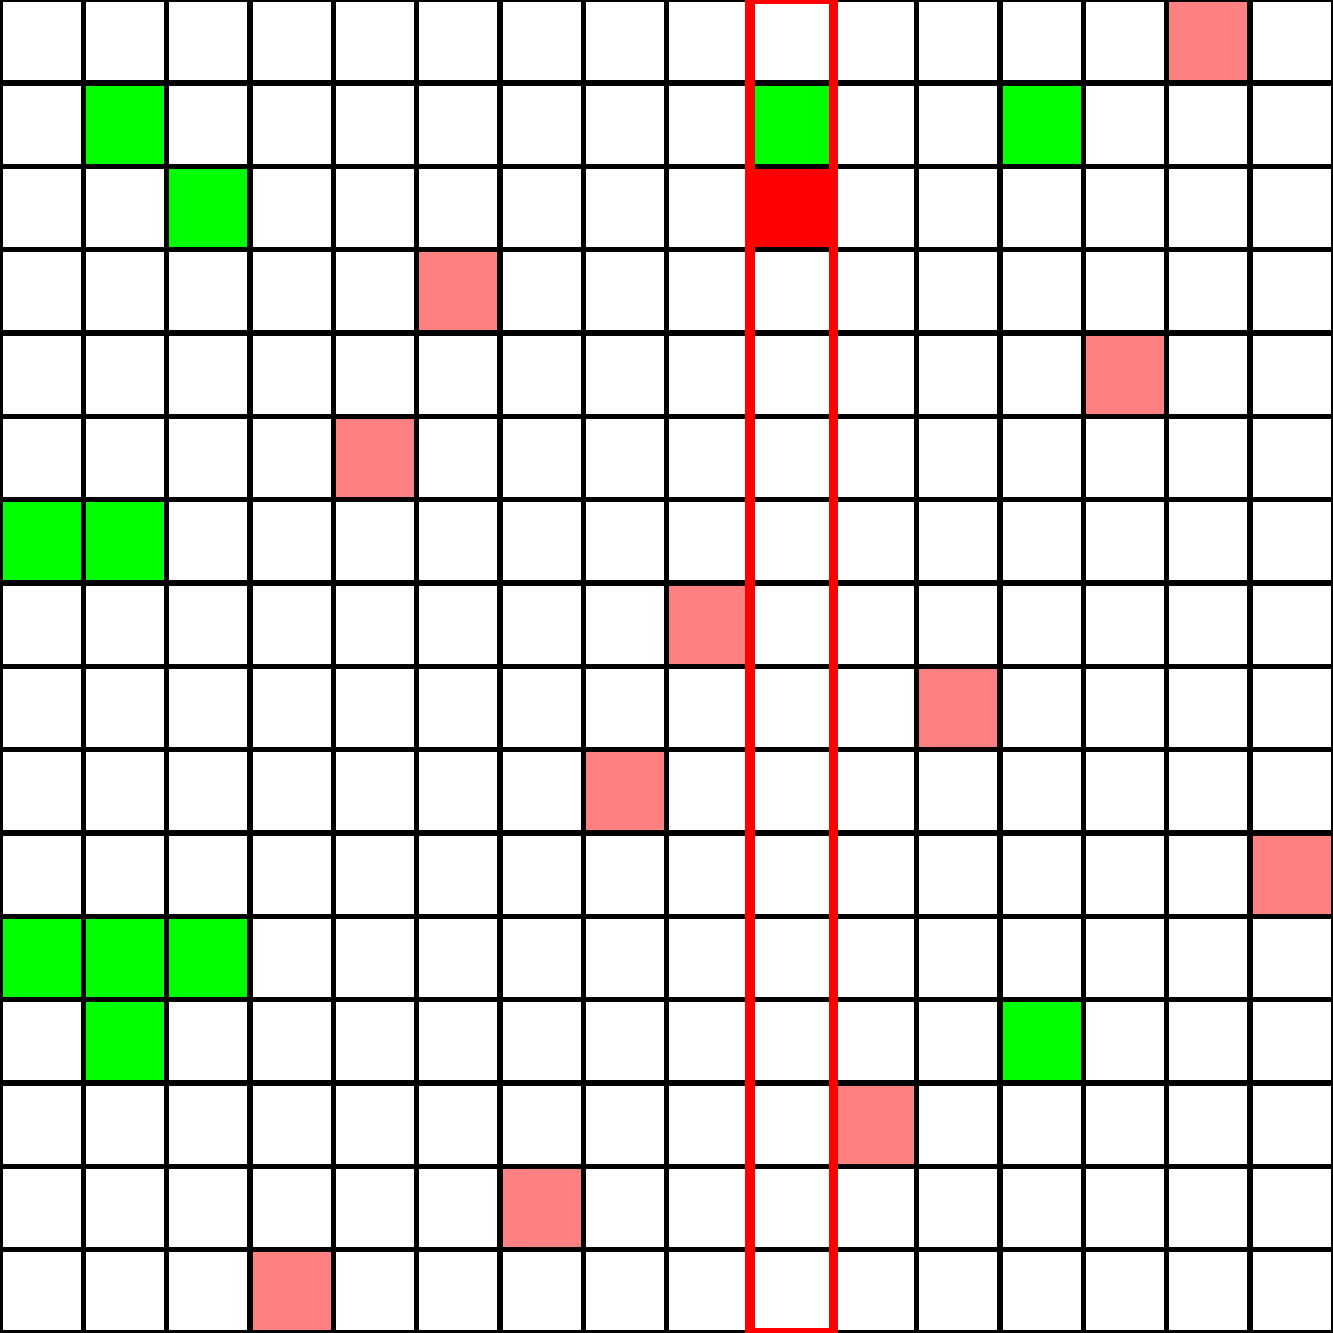
\includegraphics[width=3cm]{../nqueen/full/frame23}}
\only<24>{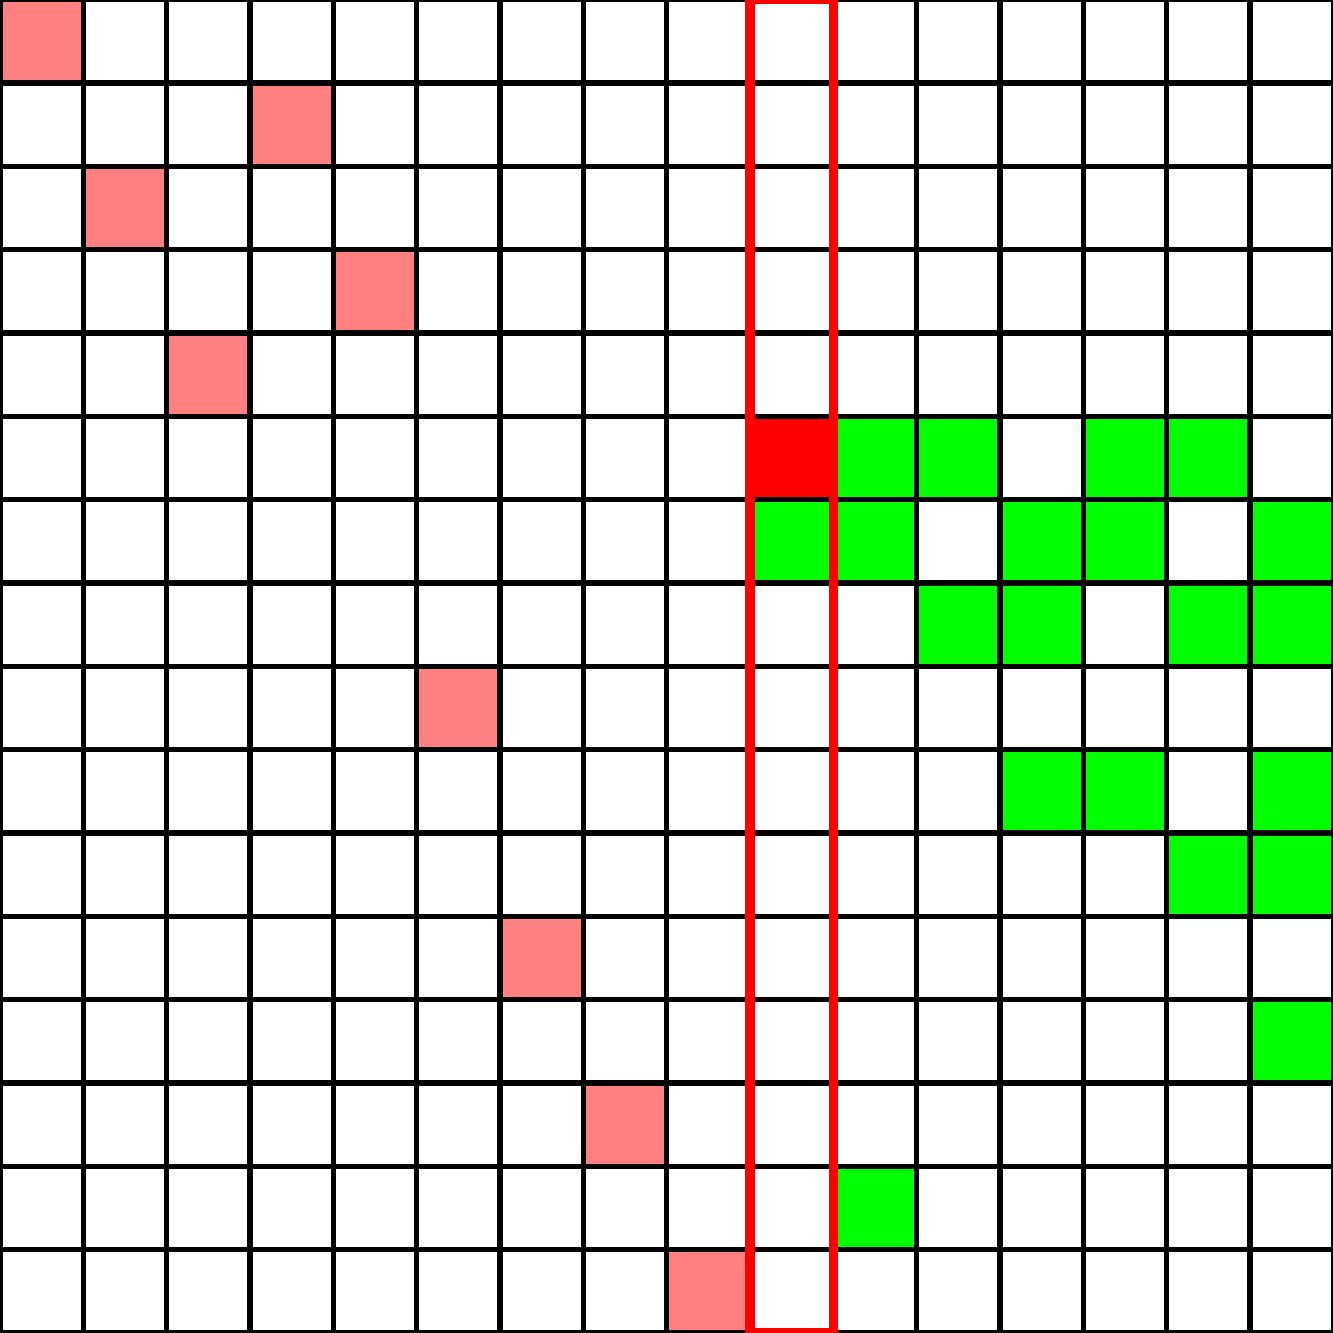
\includegraphics[width=3cm]{../nqueen/full/frame24}}
\only<25>{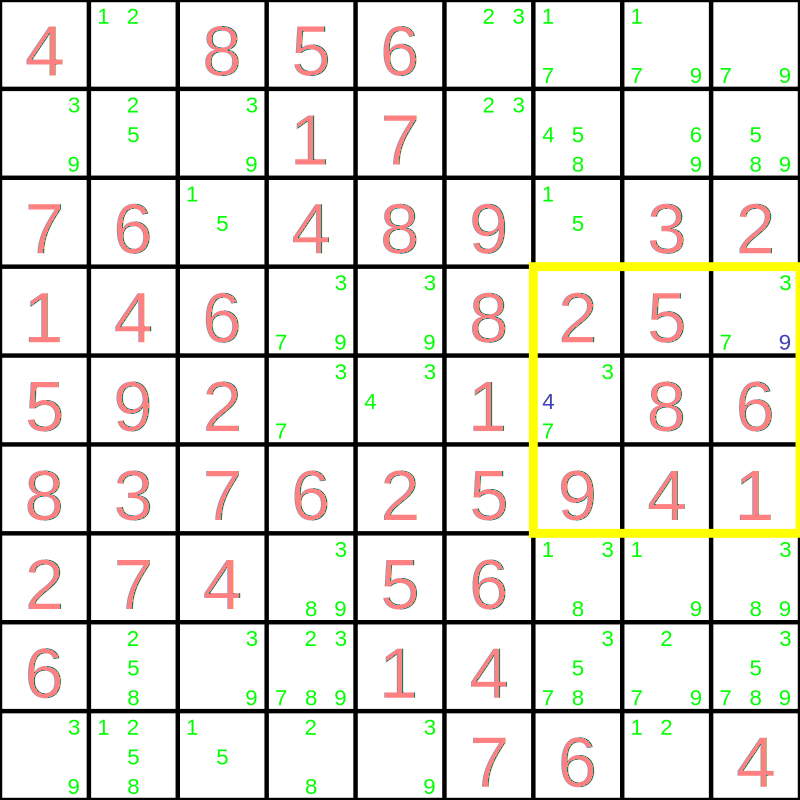
\includegraphics[width=3cm]{../nqueen/full/frame25}}
\only<26>{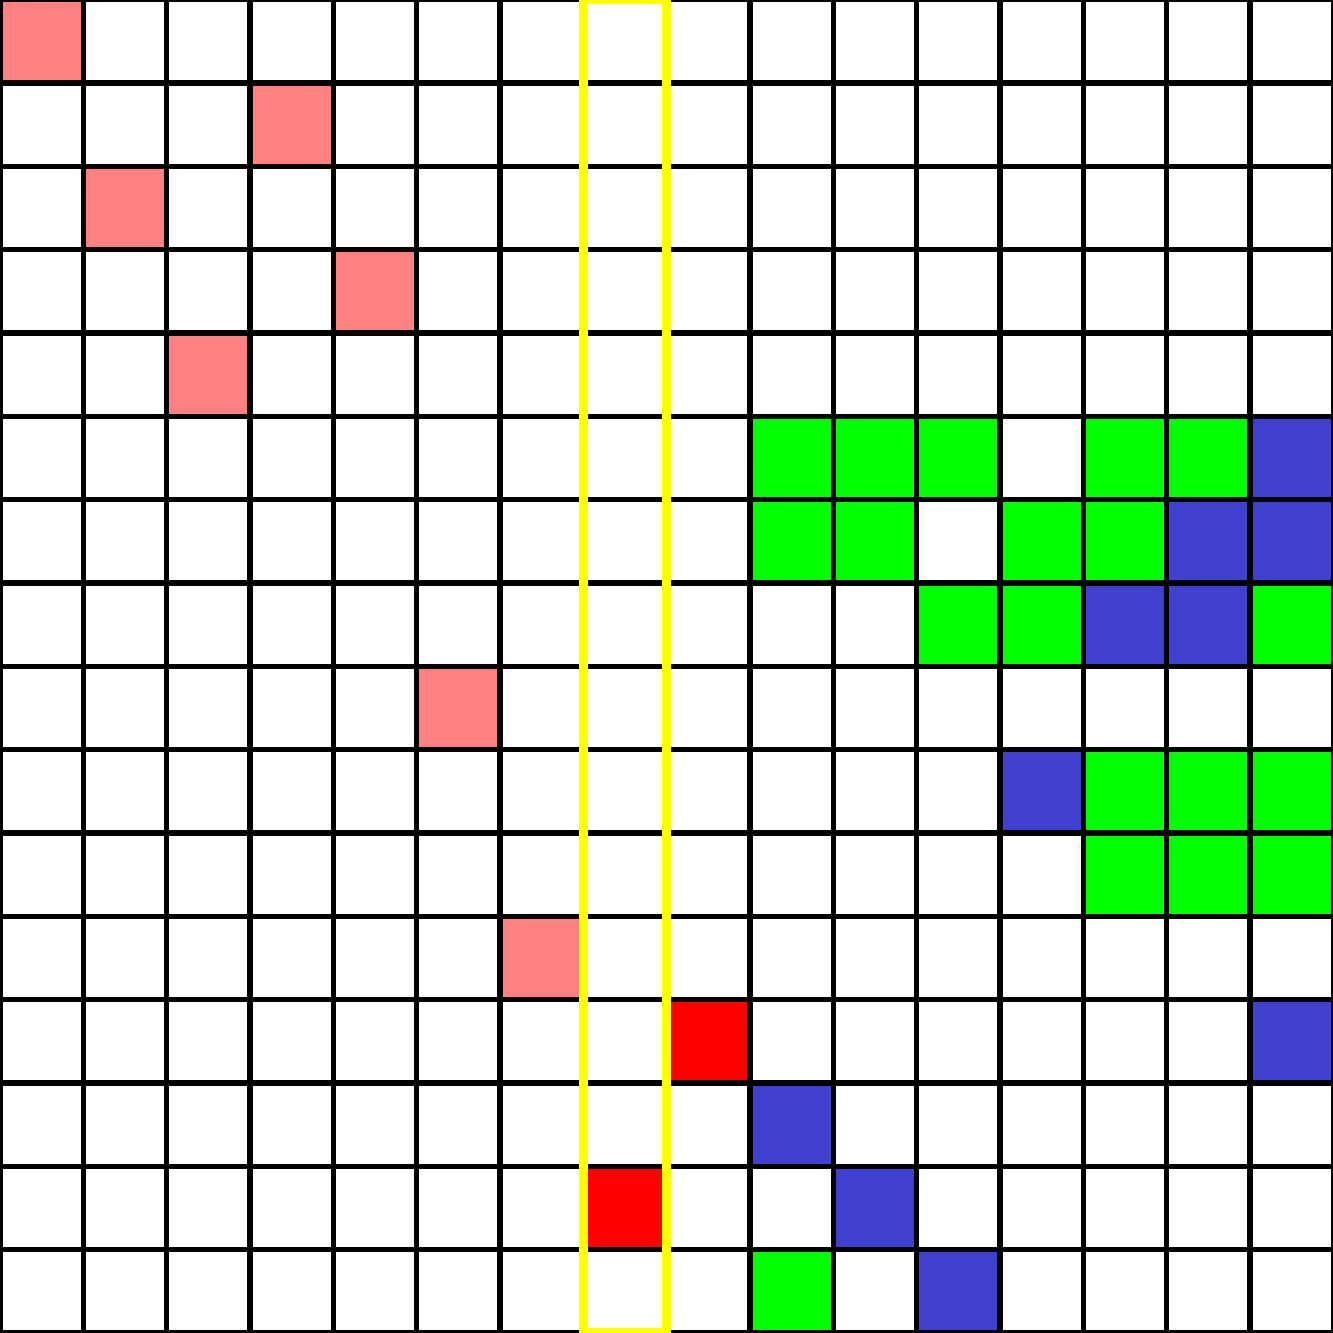
\includegraphics[width=3cm]{../nqueen/full/frame26}}
\only<27>{\includegraphics[width=3cm]{../nqueen/full/frame27}}
\only<28>{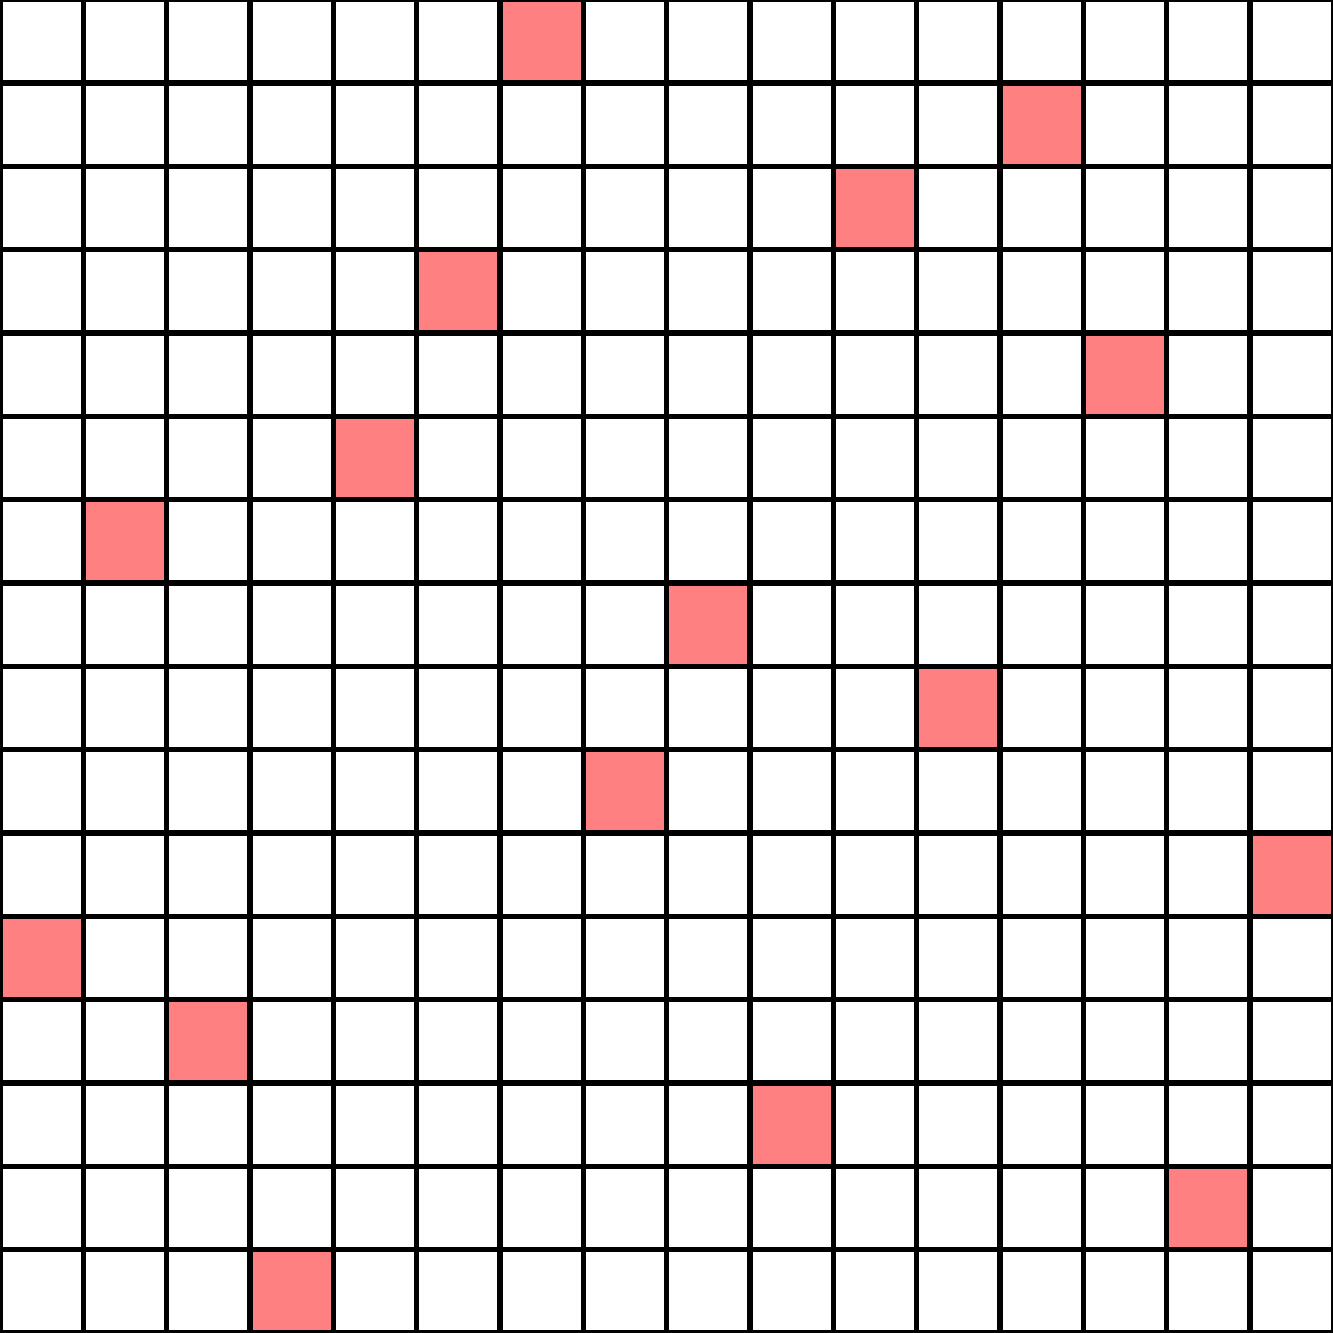
\includegraphics[width=3cm]{../nqueen/full/frame28}}
\only<29>{\includegraphics[width=3cm]{../nqueen/full/frame29}}
\only<30>{\includegraphics[width=3cm]{../nqueen/full/frame30}}
\only<31>{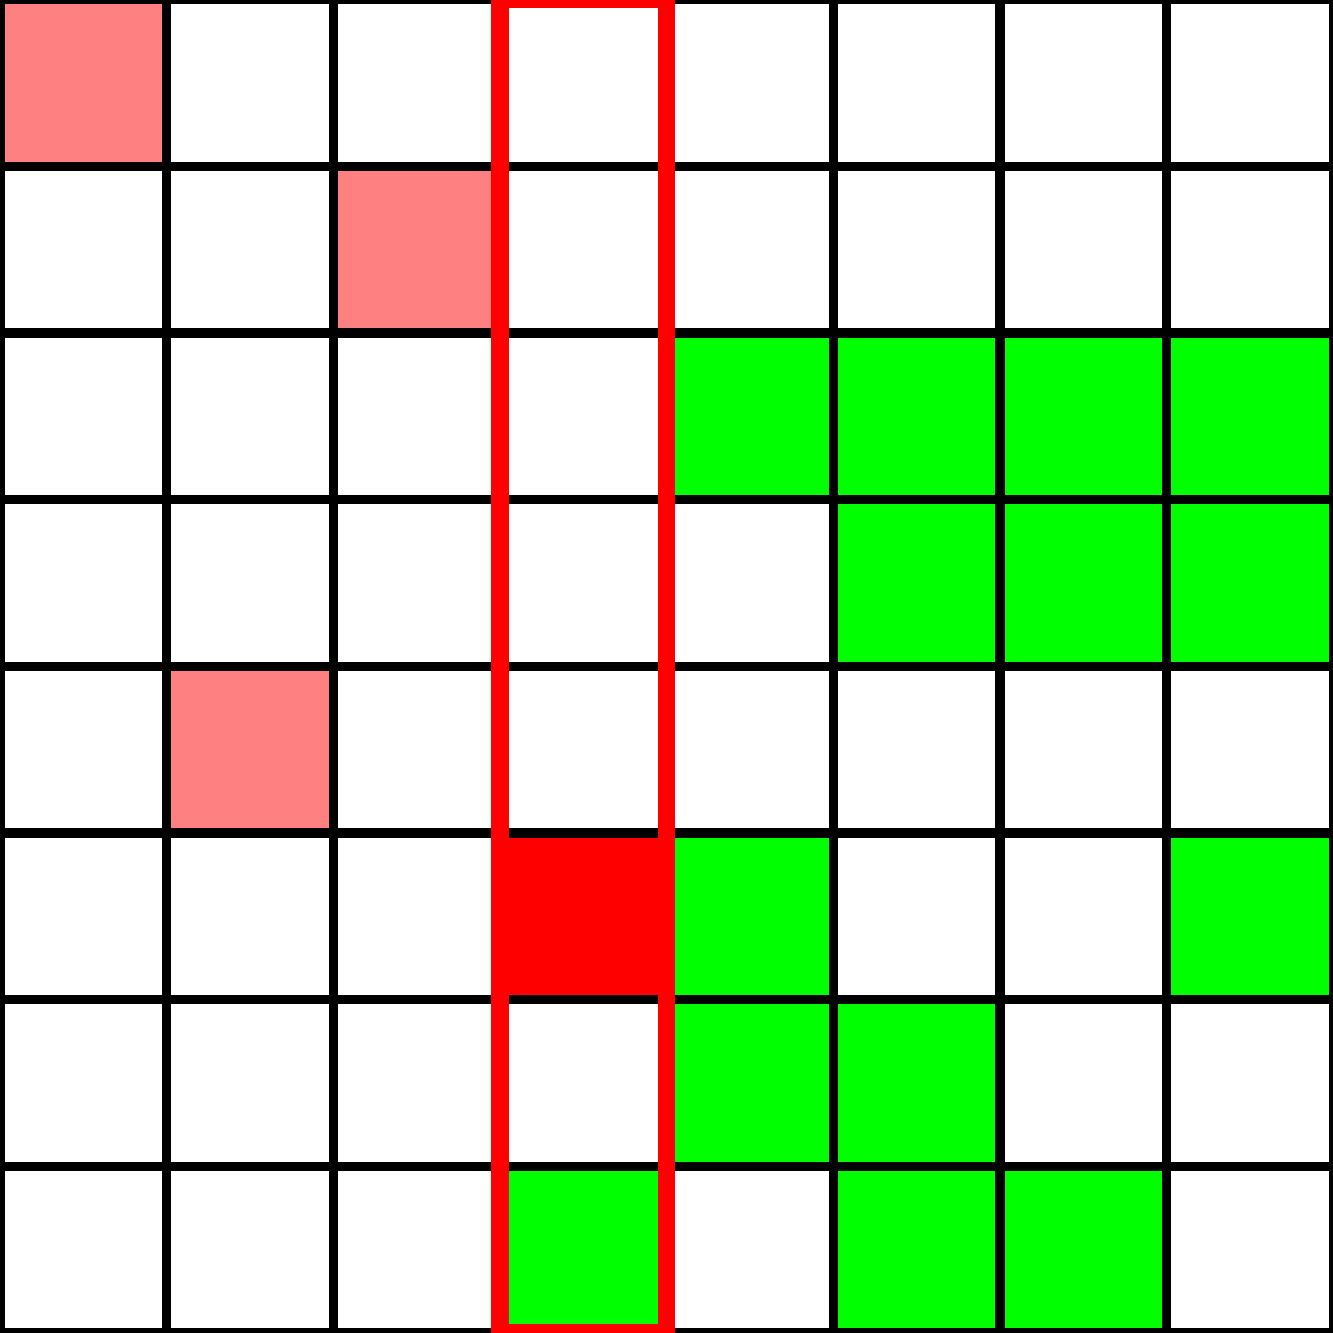
\includegraphics[width=3cm]{../nqueen/full/frame31}}
\only<32>{\includegraphics[width=3cm]{../nqueen/full/frame32}}
\only<33>{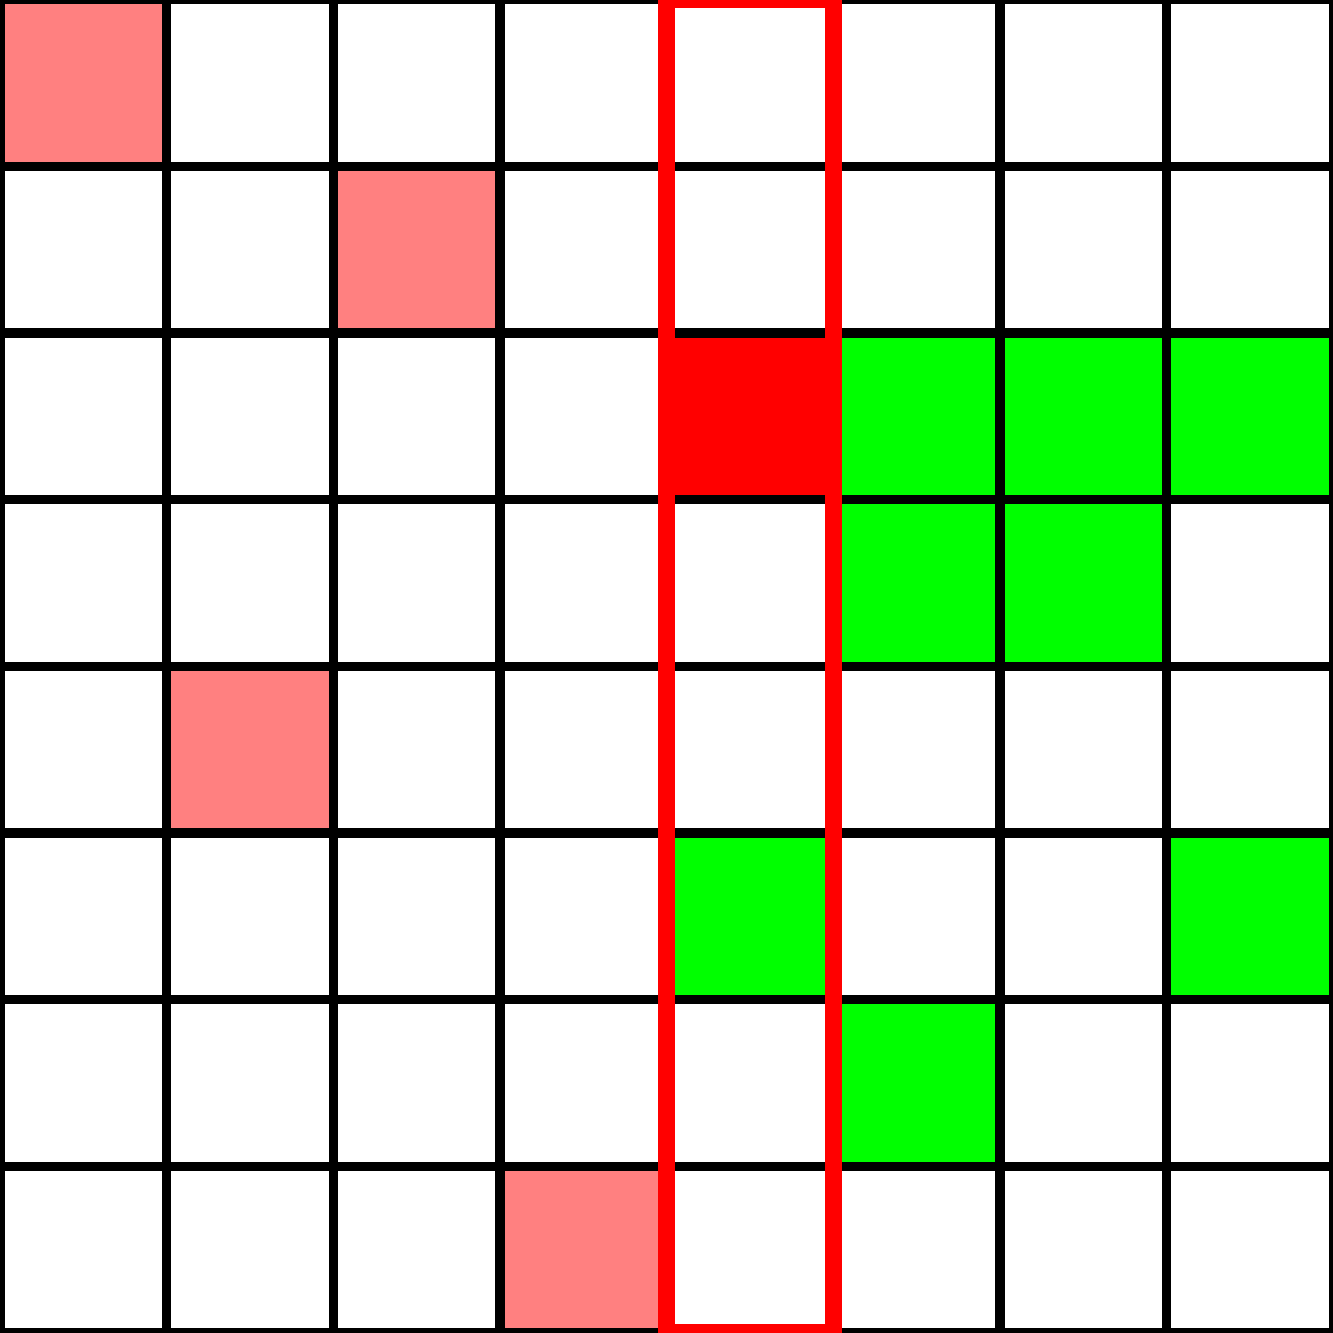
\includegraphics[width=3cm]{../nqueen/full/frame33}}
\only<34>{\includegraphics[width=3cm]{../nqueen/full/frame34}}
\only<35>{\includegraphics[width=3cm]{../nqueen/full/frame35}}
\only<36>{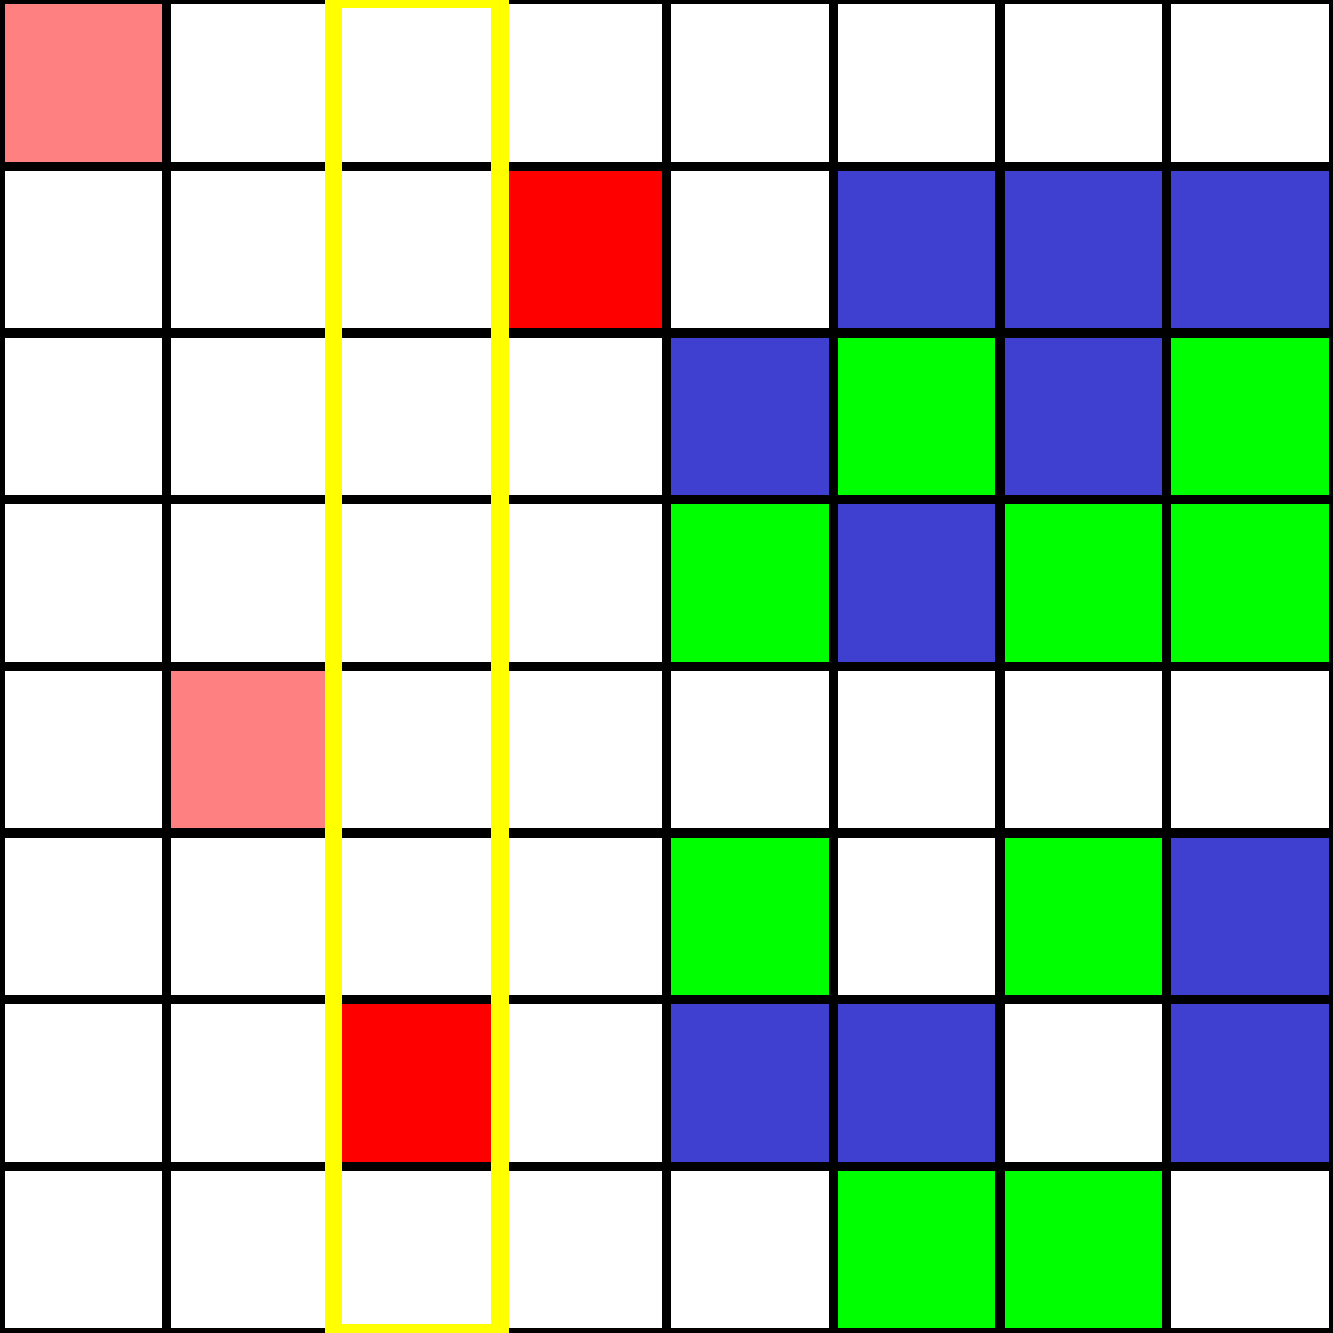
\includegraphics[width=3cm]{../nqueen/full/frame36}}
\only<37>{\includegraphics[width=3cm]{../nqueen/full/frame37}}
\only<38>{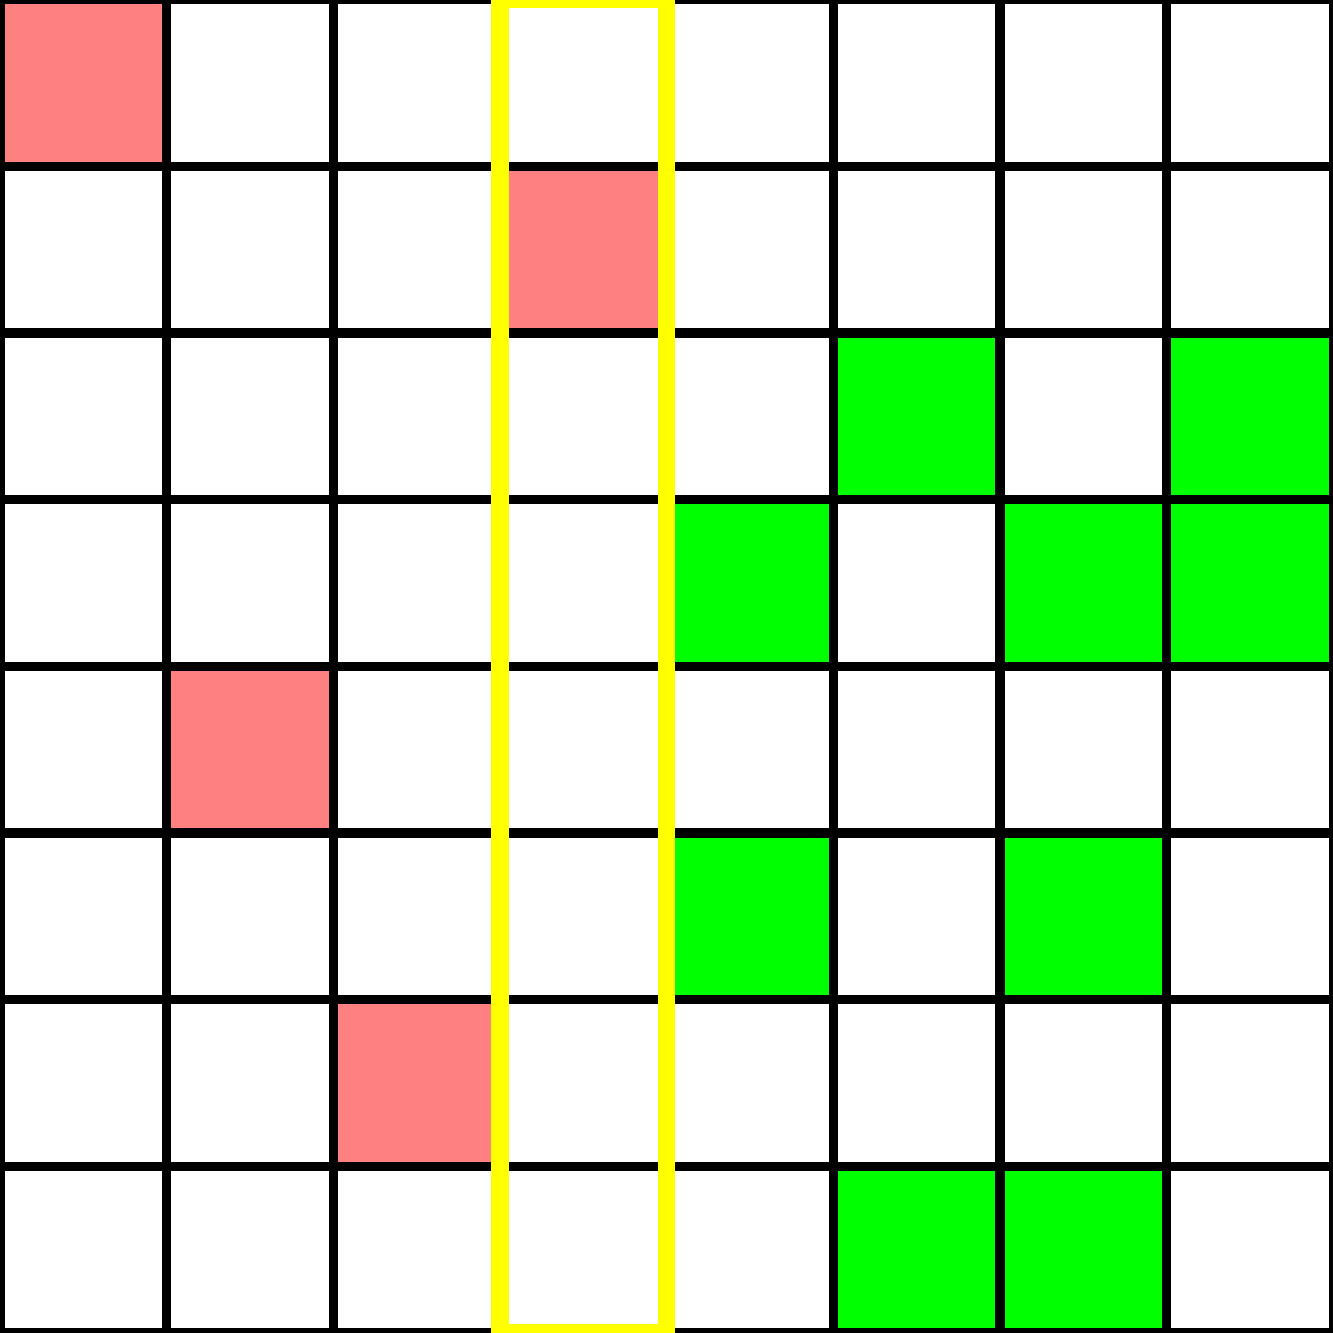
\includegraphics[width=3cm]{../nqueen/full/frame38}}
\only<39>{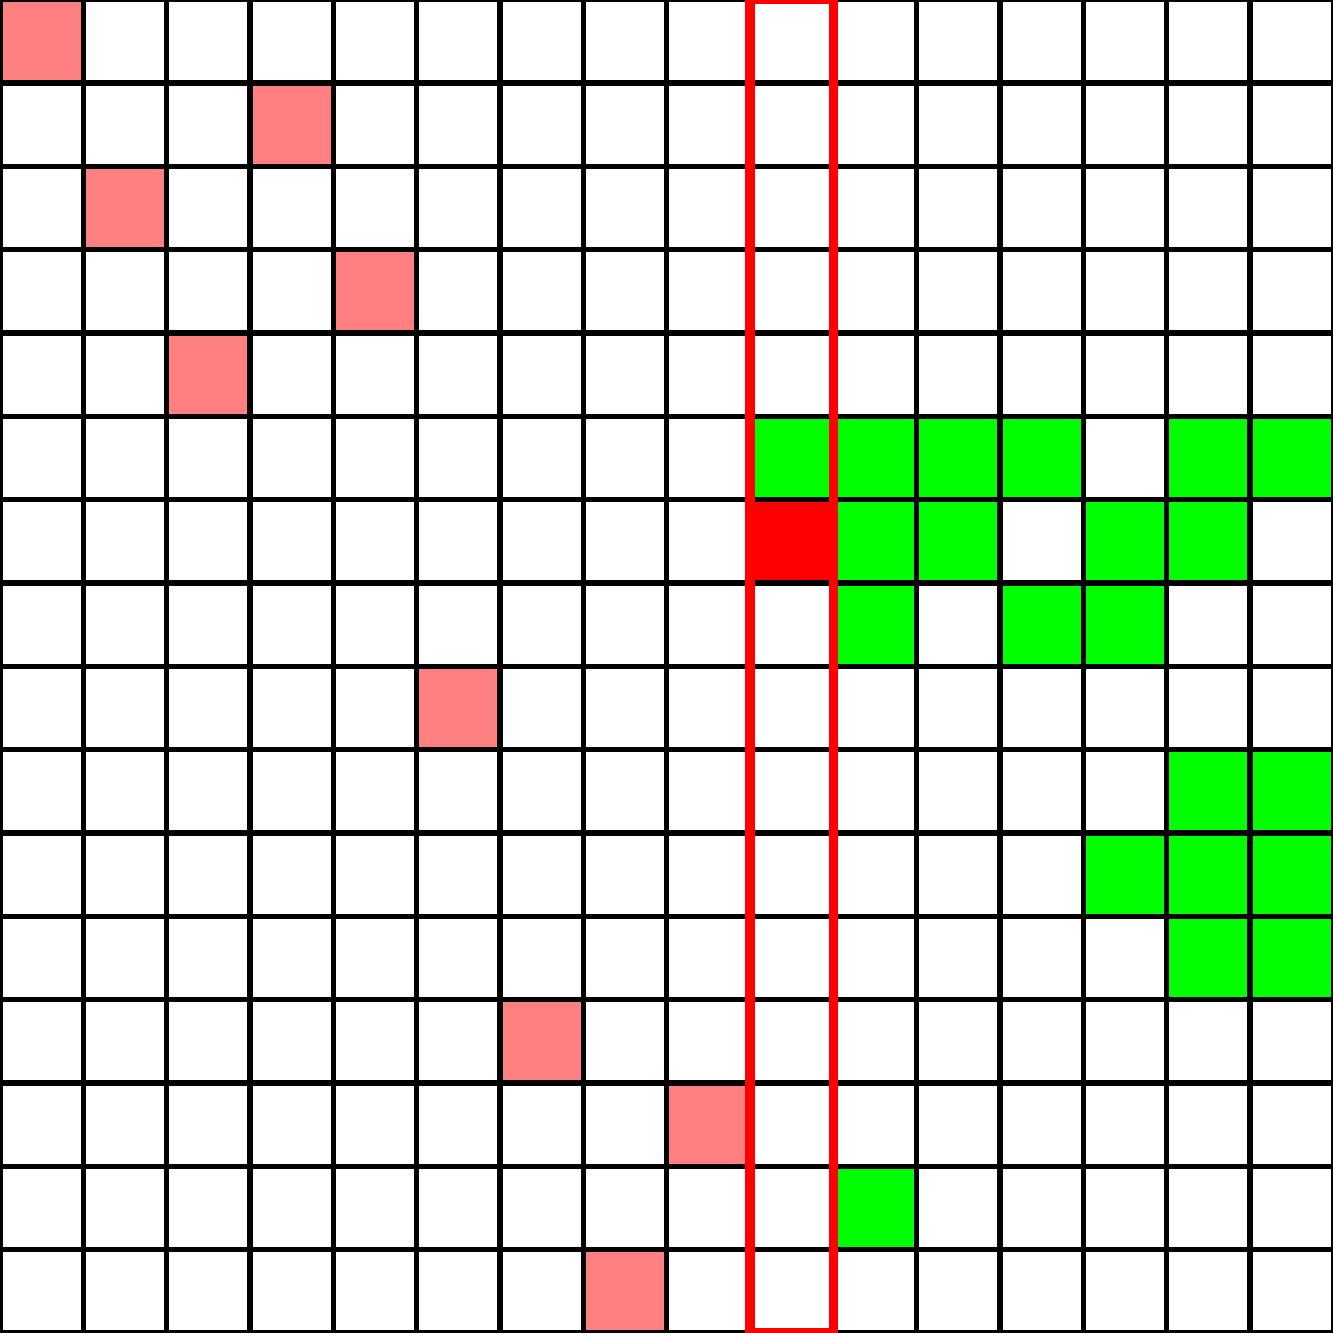
\includegraphics[width=3cm]{../nqueen/full/frame39}}
\only<40>{\includegraphics[width=3cm]{../nqueen/full/frame40}}
\only<41>{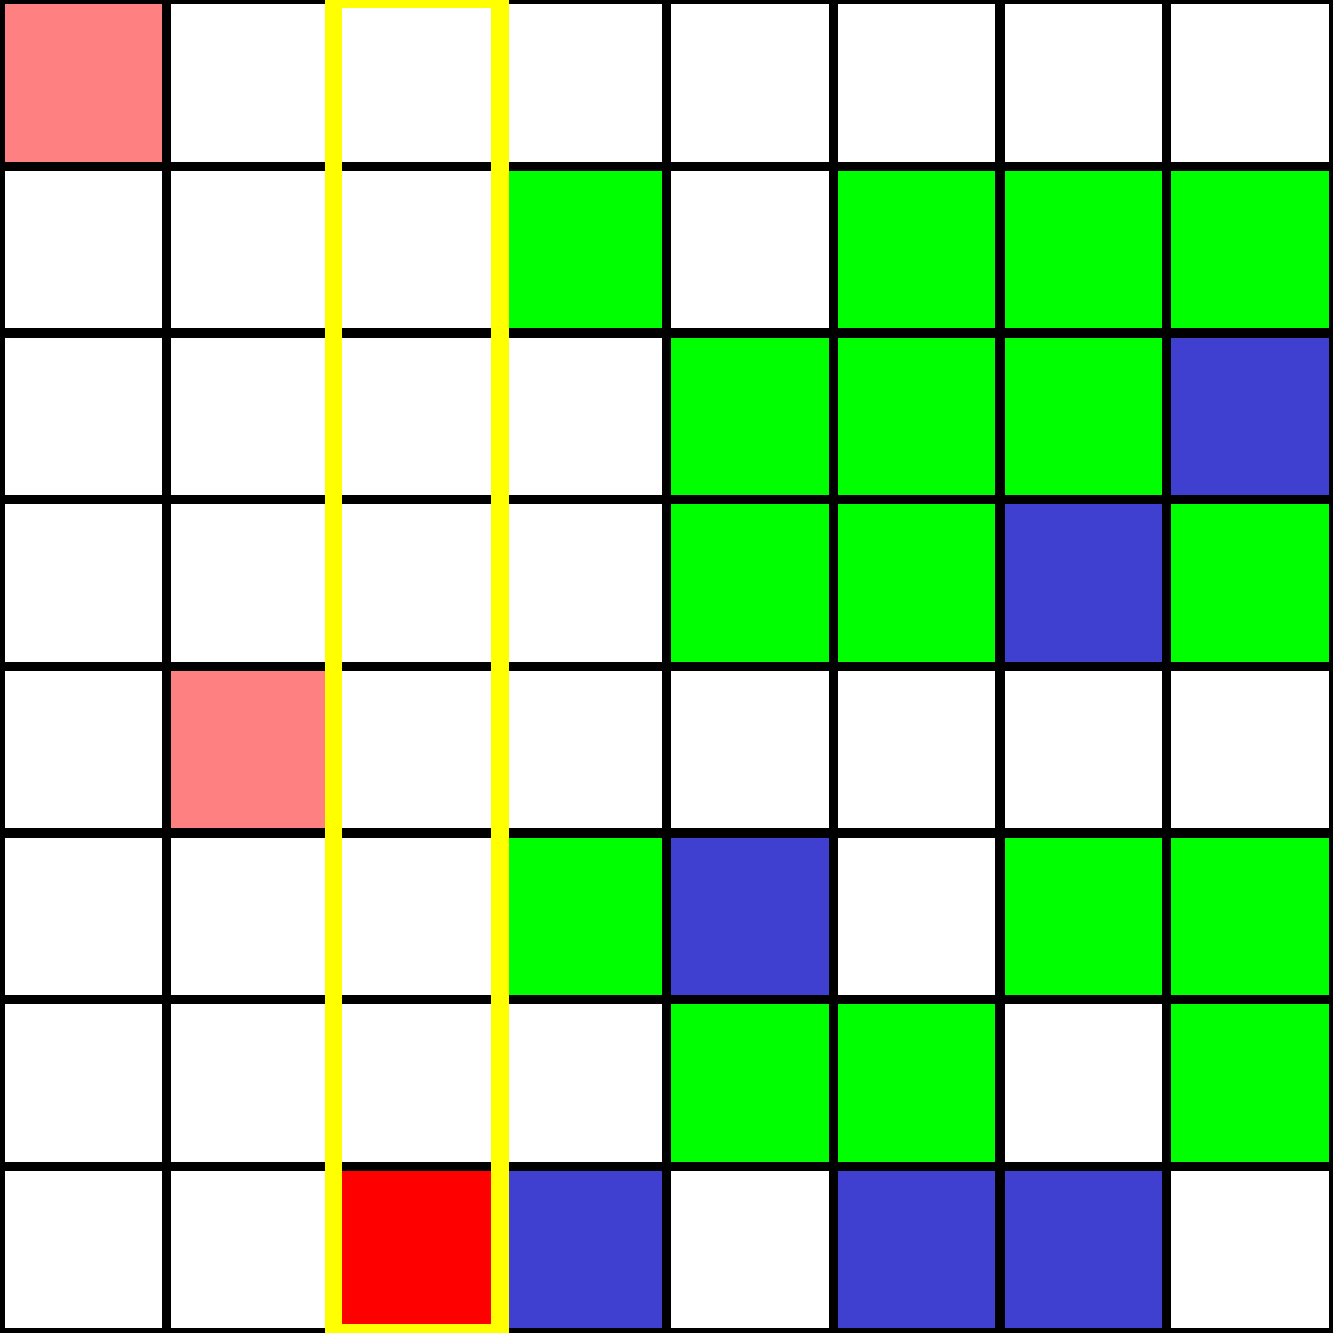
\includegraphics[width=3cm]{../nqueen/full/frame41}}
\only<42>{\includegraphics[width=3cm]{../nqueen/full/frame42}}
\only<43>{\includegraphics[width=3cm]{../nqueen/full/frame43}}
\only<44>{\includegraphics[width=3cm]{../nqueen/full/frame44}}
\only<45>{\includegraphics[width=3cm]{../nqueen/full/frame45}}
\only<46>{\includegraphics[width=3cm]{../nqueen/full/frame46}}
\only<47>{\includegraphics[width=3cm]{../nqueen/full/frame47}}
\only<48>{\includegraphics[width=3cm]{../nqueen/full/frame48}}
\only<49>{\includegraphics[width=3cm]{../nqueen/full/frame49}}
\end{textblock}
\only<1>{\includegraphics[width=6cm]{../nqueen/full/tree_expanded_1}}
\only<2>{\includegraphics[width=6cm]{../nqueen/full/tree_expanded_2}}
\only<3>{\includegraphics[width=6cm]{../nqueen/full/tree_expanded_3}}
\only<4>{\includegraphics[width=6cm]{../nqueen/full/tree_expanded_4}}
\only<5>{\includegraphics[width=6cm]{../nqueen/full/tree_expanded_5}}
\only<6>{\includegraphics[width=6cm]{../nqueen/full/tree_expanded_6}}
\only<7>{\includegraphics[width=6cm]{../nqueen/full/tree_expanded_7}}
\only<8>{\includegraphics[width=6cm]{../nqueen/full/tree_expanded_8}}
\only<9>{\includegraphics[width=6cm]{../nqueen/full/tree_expanded_9}}
\only<10>{\includegraphics[width=6cm]{../nqueen/full/tree_expanded_10}}
\only<11>{\includegraphics[width=6cm]{../nqueen/full/tree_expanded_11}}
\only<12>{\includegraphics[width=6cm]{../nqueen/full/tree_expanded_12}}
\only<13>{\includegraphics[width=6cm]{../nqueen/full/tree_expanded_13}}
\only<14>{\includegraphics[width=6cm]{../nqueen/full/tree_expanded_14}}
\only<15>{\includegraphics[width=6cm]{../nqueen/full/tree_expanded_15}}
\only<16>{\includegraphics[width=6cm]{../nqueen/full/tree_expanded_16}}
\only<17>{\includegraphics[width=6cm]{../nqueen/full/tree_expanded_17}}
\only<18>{\includegraphics[width=6cm]{../nqueen/full/tree_expanded_18}}
\only<19>{\includegraphics[width=6cm]{../nqueen/full/tree_expanded_19}}
\only<20>{\includegraphics[width=6cm]{../nqueen/full/tree_expanded_20}}
\only<21>{\includegraphics[width=6cm]{../nqueen/full/tree_expanded_21}}
\only<22>{\includegraphics[width=6cm]{../nqueen/full/tree_expanded_22}}
\only<23>{\includegraphics[width=6cm]{../nqueen/full/tree_expanded_23}}
\only<24>{\includegraphics[width=6cm]{../nqueen/full/tree_expanded_24}}
\only<25>{\includegraphics[width=6cm]{../nqueen/full/tree_expanded_25}}
\only<26>{\includegraphics[width=6cm]{../nqueen/full/tree_expanded_26}}
\only<27>{\includegraphics[width=6cm]{../nqueen/full/tree_expanded_27}}
\only<28>{\includegraphics[width=6cm]{../nqueen/full/tree_expanded_28}}
\only<29>{\includegraphics[width=6cm]{../nqueen/full/tree_expanded_29}}
\only<30>{\includegraphics[width=6cm]{../nqueen/full/tree_expanded_30}}
\only<31>{\includegraphics[width=6cm]{../nqueen/full/tree_expanded_31}}
\only<32>{\includegraphics[width=6cm]{../nqueen/full/tree_expanded_32}}
\only<33>{\includegraphics[width=6cm]{../nqueen/full/tree_expanded_33}}
\only<34>{\includegraphics[width=6cm]{../nqueen/full/tree_expanded_34}}
\only<35>{\includegraphics[width=6cm]{../nqueen/full/tree_expanded_35}}
\only<36>{\includegraphics[width=6cm]{../nqueen/full/tree_expanded_36}}
\only<37>{\includegraphics[width=6cm]{../nqueen/full/tree_expanded_37}}
\only<38>{\includegraphics[width=6cm]{../nqueen/full/tree_expanded_38}}
\only<39>{\includegraphics[width=6cm]{../nqueen/full/tree_expanded_39}}
\only<40>{\includegraphics[width=6cm]{../nqueen/full/tree_expanded_40}}
\only<41>{\includegraphics[width=6cm]{../nqueen/full/tree_expanded_41}}
\only<42>{\includegraphics[width=6cm]{../nqueen/full/tree_expanded_42}}
\only<43>{\includegraphics[width=6cm]{../nqueen/full/tree_expanded_43}}
\only<44>{\includegraphics[width=6cm]{../nqueen/full/tree_expanded_44}}
\only<45>{\includegraphics[width=6cm]{../nqueen/full/tree_expanded_45}}
\only<46>{\includegraphics[width=6cm]{../nqueen/full/tree_expanded_46}}
\only<47>{\includegraphics[width=6cm]{../nqueen/full/tree_expanded_47}}
\only<48>{\includegraphics[width=6cm]{../nqueen/full/tree_expanded_48}}
\only<49>{\includegraphics[width=6cm]{../nqueen/full/tree_expanded_49}}
\vfill
\hyperlinkframestart<2-49>{\beamerreturnbutton{Back to Start}}
\hyperlinkframeend<1-48>{\beamerskipbutton{Skip Animation}}
}
\only<handout>{
\includegraphics[width=6cm]{../nqueen/full/tree_expanded_49}
}
\end{frame}

\begin{figure}[h]
\caption{\label{nqueen:first assignment} First Assignment}
\begin{center}
\begin{tabular}[t]{cc}
\includegraphics[width=8cm]{../nqueen/full/tree_expanded_2}
&
\includegraphics[width=4cm]{../nqueen/full/frame2}
\end{tabular}
\end{center}
\end{figure}

We see (in Figure~\ref{nqueen:first assignment}) the search tree on the left, and the current partial assignment on the right. As the first assignment we have fixed $X_1$ to value 1. This is shown as a red rectangle on the board on the right, indicating the value selected. The currently assigned variable is represented by a yellow outline. The constraint propagation after the assignment has removed values from the other variables. The removed values are shown in blue, the remaining values in the domains are shown as green.

\begin{figure}[h]
\caption{\label{nqueen:second assignment} Second Assignment}
\begin{center}
\begin{tabular}{cc}
\includegraphics[width=8cm]{../nqueen/full/tree_expanded_3}
&
\includegraphics[width=4cm]{../nqueen/full/frame3}
\end{tabular}
\end{center}
\end{figure}

In the second assignment step (Figure~\ref{nqueen:second assignment}), we assign a value for variable $X_2$. We use value 3, since the values 1 and 2 have been removed from the domain by the previous assignment.

\begin{figure}[h]
\caption{\label{nqueen:third assignment} Third Assignment}
\begin{center}
\begin{tabular}{cc}
\includegraphics[width=8cm]{../nqueen/full/tree_expanded_4}
&
\includegraphics[width=4cm]{../nqueen/full/frame4}
\end{tabular}
\end{center}
\end{figure}
In the next step (Figure~\ref{nqueen:third assignment}), we encounter a problem. When we try to assign value 5 to variable $X_3$, we detect a failure in constraint propagation. This is why the variable is outlined in red on our board, it is also shown by a red leaf node in the search tree. After the failure, we backtrack to the last open choice, this is variable $X_3$, and try the next available value. In this way we continue our search, stopping whenever we detect a failure and continuing until all variables are assigned or no more choices are left.

\begin{frame}<presentation>
\frametitle{First Solution}
\begin{textblock}{4}(10,1)
\includegraphics[width=3cm]{../nqueen/full/frame50}
\end{textblock}
\includegraphics[width=9cm]{../nqueen/full/tree_expanded}
\end{frame}

\begin{figure}[h]
\caption{\label{nqueen:first solution} First Solution}
\begin{center}
\begin{tabular}{cc}
\includegraphics[width=8cm]{../nqueen/full/tree_expanded}
&
\includegraphics[width=4cm]{../nqueen/full/frame50}
\end{tabular}
\end{center}
\end{figure}

Finally (Figure~\ref{nqueen:first solution}) we find a solution after quite a few backtracking steps. On the right we see the solution found, on the left the search tree explored. Some links in the tree are shown in yellow, this means they are forced assignments made by constraint propagation. If we go back a few steps, we sees that as soon as variable $X_4$ is assigned to 6, the remaining variables are assigned by propagation, so we don't have to choose values for those variables.

\begin{frame}
\frametitle{Observations}
\begin{itemize}
\item Even for small problem size, tree can become large
\item Not interested in all details
\item Ignore all automatically fixed variables
\item For more compact representation abstract failed sub-trees
\end{itemize}
\end{frame}

What we can see is that even for small problem sizes, the search tree can become quite large. We are normally not interested in all details of the propagation and the search, so we will tell the system to ignore things like automatically fixed variables.

Sometimes we also want to have a shorter representation of the search, a tree in the form shown here may become too wide to fit on our display. In that case, we can choose a more compact representation, which compresses all failed subtrees into little red triangles.

\begin{frame}<presentation>
\frametitle{Compact Representation}
\begin{textblock}{7}(4,1)
\begin{tabular}{cc}
Number inside triangle:& Number of choices\\
Number under triangle:& Number of failures
\end{tabular}
\end{textblock}
\includegraphics[width=7cm]{../nqueen/compact/tree_compact}
\end{frame}

\begin{figure}[h]
\caption{\label{nqueen:compact} Compact Tree Presentation}
\begin{center}
\includegraphics[width=9cm]{../nqueen/compact/tree_compact}
\end{center}
\end{figure}

We get a view like this (Figure~\ref{nqueen:compact}). We have our variable $X_1$, which we assign to value 1, we then choose variable $X_2$, for which we first try value 3. This leads to a dead subtree, which does not contain any solutions. This is marked by a triangle, the number inside gives the number of interior nodes (here 4) and the number below gives the number of failures in the subtree (here 7). 

Eventually we come to a solution in the green solution node at the bottom, after having assigned four variables.


\begin{frame}
\frametitle{Exploring other board sizes}
\begin{itemize}
\item How stable is the model?
\item Try all sizes from 4 to 100
\item Timeout of 100 seconds
\end{itemize}
\end{frame}

One interesting question is ``How stable is this model?'', can we use it to solve the problem for different board sizes. To make this experiment, we try out all sizes from 4 to 100, with a timeout of 100 seconds. Board sizes 2 and 3 do not allow solutions, you may want to check this yourself on a piece of paper.

\begin{frame}<presentation>
\frametitle{Naive Stategy, Problem Sizes 4-100}
\includegraphics[width=10cm]{../nqueen/naive/all}
\end{frame}

\begin{figure}[h]
\caption{\label{nqueen:naive} Naive Stategy, Problem Sizes 4-100}
\begin{center}
\includegraphics[width=12cm]{../nqueen/naive/all}
\end{center}
\end{figure}

In Figure~\ref{nqueen:naive} we have a plot of the solutions we obtained. The board size is on the x-axis, time required on the y-axis. We see that initially, we find solutions quite rapidly, up to size 20. For larger sizes, the times vary a lot, for size 25 we use less than a second, but for size 28 we need 25 seconds. More importantly, we don't find any solutions for sizes greater than 30 within the timeout limit of 100 seconds.

\begin{frame}<presentation>
\frametitle{Observations}
\begin{itemize}
\item Time very reasonable up to size 20
\item Sizes 20-30 times very variable
\item Not just linked to problem size
\item No size greater than 30 solved within timeout
\end{itemize}
\end{frame}

This problem is not just linked to problem size. We would expect the program to take longer for a bigger board, but this is not a simple monotonic function. Some problem sizes require much more time to solve than others. What can we do about this?

\clearpage
\section{Improvements}
\subsection{Dynamic Variable Choice}

Can we do better than our naive, straighforward program?

\begin{frame}
\frametitle{Possible Improvements}
\begin{itemize}
\item Better constraint reasoning
\begin{itemize}
\item Remodelling problem with 3 \texttt{alldifferent} constraints
\item Global reasoning as described before
%\item Not explored here
\end{itemize}
\item Better control of search
\begin{itemize}
\item Static vs. dynamic variable ordering
\item Better value choice
\item Not using complete depth-first chronological backtracking
\end{itemize}
\end{itemize}
\end{frame}

There are two ways of improving the situation. One would use better constraint reasoning, so that we detect failures earlier and do not have to explore large, dead subtrees. A way to do this is to remodel our problem with three \texttt{alldifferent} constraints, and to use the stronger consistency methods that we have explored in the previous chapter. This is not working that well for this problem, and we do not explore this here.

A more promising alternative is to improve our control of the search, introducing a dynamic instead of a static variable ordering. We can also use a better value choice, selecting a more promising value for the selected variable. Finally, we can replace our complete, chronological backtracking search with a more appropriate method.

\begin{frame}
\frametitle{Static vs. Dynamic Variable Ordering}
\begin{itemize}
\item Heuristic Static Ordering
\begin{itemize}
\item Sort variables before search based on heuristic
\item Most important decisions
\item Smallest initial domain
\end{itemize} 
\item Dynamic variable ordering
\begin{itemize}
\item Use information from constraint propagation
\item Different orders in different parts of search tree
\item Use all information available
\end{itemize}
\end{itemize}
\end{frame}

We can improve the search routine by either sorting the variables before the search is started based on a heuristic, static ordering or by using a dynamic variable ordering during search, or indeed by a combination of both methods.

For a static ordering, the idea is to make important decisions early in the search, i.e. to choose those variables which have the biggest impact on the search. By making these choices early, we reduce the problem size as quickly as possible. We can also try to assign the variables with small domains first, so that we have fewer alternative branches to explore at the top of the tree. The drawback of such a static heuristic is that we make rather uninformed choices. We can only use the information available at the beginning of the program.

It is usually much better to make the variable selection choice dynamically, this way we can use the current state of the propagation to guide our choice. This can also mean that we use a different ordering in one part of the search tree from the one in another part of the tree. This way we use all information available at every step.

\begin{frame}
\frametitle{First Fail strategy}
\begin{itemize}
\item Dynamic variable ordering
\item At each step, select variable with smallest domain
\item Idea: If there is a solution, better chance of finding it
\item Idea: If there is no solution, smaller number of alternatives
\item Needs tie-breaking method
\end{itemize}
\end{frame}

One such dynamic selection method is the first fail strategy. At each step, we select the variable which has the smallest domain. There are typically two justifications given for this: 
\begin{itemize}
\item If there are very few solutions, we have a better chance of finding it by branching on few alternatives. 
\item If there are no solutions, then we have fewer alternatives to explore, and this should require less time than choosing a variable with a large domain, and exploring many alternatives.
\end{itemize}
This first fail principle needs a tie-breaking method, to decide what to do if several variables have the same, smallest domain size. In ECLiPSe, we typically use the first variable which has the smallest domain.

\begin{frame}
\frametitle{Search Stategy Choices}
\begin{itemize}
\item Minizinc \hyperlink{nqueens:minizinc mod}{\beamergotobutton{Show}}
\item Choco-solver \hyperlink{nqueens:choco mod}{\beamergotobutton{Show}}
\end{itemize}
\end{frame}


\begin{frame}[fragile]
  \frametitle{Modified MiniZinc Program}
  \label{nqueens:minizinc mod}
  \small
  \begin{semiverbatim}
int: n=8;
array[1..n] of var 1..n: queens;
constraint
    forall(i, j in 1..n where i < j) (
         queens[i] != queens[j] /\\
         queens[i] + i != queens[j] + j /\\
         queens[i] - i != queens[j] - j
    )
 ;
solve :: int\_search(
        queens,
        \textbf{first\_fail},
        indomain\_min)
        satisfy;
  \end{semiverbatim}

\end{frame}

\begin{frame}
\frametitle{Variable Choice (MiniZinc)}
\begin{itemize}
\item Determines the order in which variables are assigned
\item \texttt{input\_order} assign variables in static order given
\item \texttt{smallest} assign variable with smallest value in domain first
\item \texttt{first\_fail} select variable with smallest domain first
\item \texttt{dom\_w\_deg} consider ratio of domain size and failure count
\item Others, including programmed selection for specific solvers
\end{itemize}
\end{frame}


\begin{frame}
\frametitle{Value Choice (MiniZinc)}
\begin{itemize}
\item Determines the order in which values are tested for selected variables
\item \texttt{indomain\_min} Start with smallest value, on backtracking try next larger value
\item \texttt{indomain\_median} Start with value closest to middle of domain
\item \texttt{indomain\_random} Choose values in random order
\item \texttt{indomain\_split} Split domain into two intervals
\end{itemize}
  \hyperlink{nqueens:continue mod}{\beamergotobutton{Continue}}
\end{frame}


\begin{frame}[fragile]
\frametitle{Modified Choco-solver Model}
\label{nqueens:choco mod}
\tiny
\begin{verbatim}
int n = 8;

Model model = new Model(n + "-queens problem");
IntVar[] vars = model.intVarArray("Q", n, 1, n, false);
IntVar[] diag1 = IntStream.range(0, n).
                           mapToObj(i -> vars[i].sub(i).intVar()).
                           toArray(IntVar[]::new);
IntVar[] diag2 = IntStream.range(0, n).
                           mapToObj(i -> vars[i].add(i).intVar()).
                           toArray(IntVar[]::new);
                           
model.post(
    model.allDifferent(vars),
    model.allDifferent(diag1),
    model.allDifferent(diag2)
);

Solver solver = model.getSolver();
solver.showStatistics();
solver.setSearch(Search.domOverWDegSearch(vars));
Solution solution = solver.findSolution();

if (solution != null) {
    System.out.println(solution.toString());
}
\end{verbatim}
\end{frame}

\begin{frame}
\frametitle{VariableSelector Choice (Choco-solver)}
\begin{itemize}
\item Determines the order in which variables are assigned
\item \texttt{InputOrder} assign variables in static order given
\item \texttt{Smallest} assign variable with smallest value in domain first
\item \texttt{FirstFail} select variable with smallest domain first
\item \texttt{DomOverWDeg} consider ratio of domain size and failure count
\item \texttt{ActivityBased} dynamic, based on dynamic observed behaviour
\item \texttt{ImpactBased} dynamic, based on dynamic observed behaviour
\end{itemize}
\end{frame}


\begin{frame}
\frametitle{IntValueSelector Choice (Choco-solver)}
\begin{itemize}
\item Determines the order in which values are tested for selected variables
\item \texttt{IntDomainMin} Start with smallest value, on backtracking try next larger value
\item \texttt{IntDomainMiddle} Start with value closest to middle of domain
\item \texttt{IntDomainRandom} Choose values in random order
\item \texttt{IntDomainRandomBound} Randomly choose between smallest and largest value
\end{itemize}
  \hyperlink{nqueens:continue mod}{\beamergotobutton{Continue}}
\end{frame}



What changes are required to use the first fail princple in our example problem? We have to replace the \texttt{labeling} routine with a more general method, the \texttt{search} builtin of the ic library, where we give the list of variables to assign, and then a whole set of parameters.

 

\begin{frame}
\frametitle{Comparison}
\label{nqueens:continue mod}
\begin{itemize}
\item Board size 16x16
\item Naive (Input Order) Strategy
\item First Fail variable selection
\end{itemize}
\end{frame}

If we want to see how these methods compare, we should use a bigger problem size than the $8\times 8$ board. For demonstration purposes, we use the $16\times 16$ board. We start with the naive method, \texttt{input\_order} and \texttt{indomain} and compare it to the \texttt{first\_fail} strategy.

\begin{frame}<presentation>
\frametitle{Naive (Input Order) Strategy (Size 16)}
\begin{textblock}{4}(10,1)
\includegraphics[width=3cm]{../nqueen/naive/frame2959}
\end{textblock}
\includegraphics[width=7cm]{../nqueen/naive/tree_compact}
\end{frame}

\begin{figure}[h]
\caption{\label{nqueen:naive16tree}Naive (Input Order) Strategy (Size 16) Search Tree}
\begin{center}
\includegraphics[width=12cm]{../nqueen/naive/tree_compact}
\end{center}
\end{figure}

This (Figure~\ref{nqueen:naive16tree}) is the search tree required for the naive method. This does not look too bad, until you check the size of the failed sub-trees. For variable $X_5$ we explore 6 failed alternatives with hundreds of failures each, before we make the correct choice.

\begin{frame}<presentation>
\frametitle{FirstFail Strategy (Size 16)}
\only<beamer>{
\begin{textblock}{4}(10,1)
\only<1>{\includegraphics[width=3cm]{../nqueen/first_fail/frame1}}
\only<2>{\includegraphics[width=3cm]{../nqueen/first_fail/frame2}}
\only<3>{\includegraphics[width=3cm]{../nqueen/first_fail/frame3}}
\only<4>{\includegraphics[width=3cm]{../nqueen/first_fail/frame4}}
\only<5>{\includegraphics[width=3cm]{../nqueen/first_fail/frame5}}
\only<6>{\includegraphics[width=3cm]{../nqueen/first_fail/frame6}}
\only<7>{\includegraphics[width=3cm]{../nqueen/first_fail/frame7}}
\only<8>{\includegraphics[width=3cm]{../nqueen/first_fail/frame8}}
\only<9>{\includegraphics[width=3cm]{../nqueen/first_fail/frame9}}
\only<10>{\includegraphics[width=3cm]{../nqueen/first_fail/frame10}}
\only<11>{\includegraphics[width=3cm]{../nqueen/first_fail/frame11}}
\only<12>{\includegraphics[width=3cm]{../nqueen/first_fail/frame12}}
\only<13>{\includegraphics[width=3cm]{../nqueen/first_fail/frame13}}
\only<14>{\includegraphics[width=3cm]{../nqueen/first_fail/frame14}}
\only<15>{\includegraphics[width=3cm]{../nqueen/first_fail/frame15}}
\only<16>{\includegraphics[width=3cm]{../nqueen/first_fail/frame16}}
\only<17>{\includegraphics[width=3cm]{../nqueen/first_fail/frame17}}
\only<18>{\includegraphics[width=3cm]{../nqueen/first_fail/frame18}}
\only<19>{\includegraphics[width=3cm]{../nqueen/first_fail/frame19}}
\only<20>{\includegraphics[width=3cm]{../nqueen/first_fail/frame20}}
\only<21>{\includegraphics[width=3cm]{../nqueen/first_fail/frame21}}
\only<22>{\includegraphics[width=3cm]{../nqueen/first_fail/frame22}}
\only<23>{\includegraphics[width=3cm]{../nqueen/first_fail/frame23}}
\end{textblock}
\only<1>{\includegraphics[width=6cm]{../nqueen/first_fail/tree_expanded_1}}
\only<2>{\includegraphics[width=6cm]{../nqueen/first_fail/tree_expanded_2}}
\only<3>{\includegraphics[width=6cm]{../nqueen/first_fail/tree_expanded_3}}
\only<4>{\includegraphics[width=6cm]{../nqueen/first_fail/tree_expanded_4}}
\only<5>{\includegraphics[width=6cm]{../nqueen/first_fail/tree_expanded_5}}
\only<6>{\includegraphics[width=6cm]{../nqueen/first_fail/tree_expanded_6}}
\only<7>{\includegraphics[width=6cm]{../nqueen/first_fail/tree_expanded_7}}
\only<8>{\includegraphics[width=6cm]{../nqueen/first_fail/tree_expanded_8}}
\only<9>{\includegraphics[width=6cm]{../nqueen/first_fail/tree_expanded_9}}
\only<10>{\includegraphics[width=6cm]{../nqueen/first_fail/tree_expanded_10}}
\only<11>{\includegraphics[width=6cm]{../nqueen/first_fail/tree_expanded_11}}
\only<12>{\includegraphics[width=6cm]{../nqueen/first_fail/tree_expanded_12}}
\only<13>{\includegraphics[width=6cm]{../nqueen/first_fail/tree_expanded_13}}
\only<14>{\includegraphics[width=6cm]{../nqueen/first_fail/tree_expanded_14}}
\only<15>{\includegraphics[width=6cm]{../nqueen/first_fail/tree_expanded_15}}
\only<16>{\includegraphics[width=6cm]{../nqueen/first_fail/tree_expanded_16}}
\only<17>{\includegraphics[width=6cm]{../nqueen/first_fail/tree_expanded_17}}
\only<18>{\includegraphics[width=6cm]{../nqueen/first_fail/tree_expanded_18}}
\only<19>{\includegraphics[width=6cm]{../nqueen/first_fail/tree_expanded_19}}
\only<20>{\includegraphics[width=6cm]{../nqueen/first_fail/tree_expanded_20}}
\only<21>{\includegraphics[width=6cm]{../nqueen/first_fail/tree_expanded_21}}
\only<22>{\includegraphics[width=6cm]{../nqueen/first_fail/tree_expanded_22}}
\only<23>{\includegraphics[width=6cm]{../nqueen/first_fail/tree_expanded_23}}
\vfill
\hyperlinkframestart<2-23>{\beamerreturnbutton{Back to Start}}
\hyperlinkframeend<1-22>{\beamerskipbutton{Skip Animation}}
}
\only<handout>{
\includegraphics[width=6cm]{../nqueen/first_fail/tree_expanded_23}
}
\end{frame}

\begin{figure}[h]
\caption{\label{nqueen:ff fourth assignment} First Fail, Fourth Assignment}
\begin{center}
\begin{tabular}{cc}
\includegraphics[width=8cm]{../nqueen/first_fail/tree_expanded_5}
&
\includegraphics[width=4cm]{../nqueen/first_fail/frame5}
\end{tabular}
\end{center}
\end{figure}
This (Figure~\ref{nqueen:ff fourth assignment}) is the fourth assignment step in our modified program, and we can see that instead of variable $X_4$ the program selects $X_6$ for assignment. From there, the search differs dramatically from the naive method.

\begin{figure}[h]
\caption{\label{nqueen:firstfailtree}FirstFail Strategy (Size 16)}
\begin{center}
\includegraphics[width=12cm]{../nqueen/first_fail/tree_expanded_23}
\end{center}
\end{figure}

If we look at the complete tree for the first fail strategy (Figure~\ref{nqueen:firstfailtree}), we see it is much smaller, requiring only 7 failures before finding a solution. 

Also note that the variable order differs in the branches of the tree; on the left side, variable 7 is selected just before the failure, on the right side variable 14 is selected at that level.
 
\begin{frame}<presentation>
\frametitle{Comparing Solutions}
\begin{tabular}{cc}
Naive & First Fail \\
\includegraphics[width=4cm]{../nqueen/naive/frame2959}
&
\includegraphics[width=4cm]{../nqueen/first_fail/frame24}
\end{tabular}

\only<2>{Solutions are different!}
\end{frame}

\begin{figure}[h]
\caption{\label{nqueen:different solutions}Solutions are different!}
\begin{center}
\begin{tabular}{cc}
Naive & First Fail \\
\includegraphics[width=6cm]{../nqueen/naive/frame2959}
&
\includegraphics[width=6cm]{../nqueen/first_fail/frame24}
\end{tabular}
\end{center}
\end{figure}

It is also important to note that the solutions obtained by the two programs are different, as shown in figure~\ref{nqueen:different solutions}. We might be just lucky finding a solution earlier with first fail than the naive method.

For this problem we don't care which solution we obtain, we only look for a feasible solution, which satisfies all constraints. For other problems, we may be interested in optimizing a cost function. In that case it is important to generate the feasible solutions in a good order, finding solutions with low cost early on.

\begin{frame}<presentation>
\frametitle{FirstFail, Problem Sizes 4-100}
\includegraphics[width=10cm]{../nqueen/first_fail/all}
\end{frame}

\begin{figure}[h]
\caption{\label{nqueen:firstfail} FirstFail, Problem Sizes 4-100}
\begin{center}
\includegraphics[width=12cm]{../nqueen/first_fail/all}
\end{center}
\end{figure}

We again test our program on all instances from 4 to 100. Here (Figure~\ref{nqueen:firstfail}) we have the plot of the execution times required. This is much better than before, note the different time scale on the left. We often find solutions nearly instantly, right up to size 100. But there are still some problems which are more difficult to solve. We still don't find solutions for sizes 88, 91, 93, 97, 98, 99 within the 100 second time limit.

Using the dynamic variable selection with the first fail strategy was a very successful idea, but it does not solve the problem completely.

\begin{frame}<presentation>
\frametitle{Observations}
\begin{itemize}
\item This is much better
\item But some sizes are much harder
\item Timeout for sizes 88, 91, 93, 97, 98, 99
\end{itemize}
\end{frame}

\clearpage
\subsection{Weighted Degree}

\begin{frame}
  \frametitle{More Reactive Variable Selection}
  \begin{itemize}
  \item Domain size is important, but other information is useful as well
  \item Dom/Weighted Degree: better results in many situations
  \item Weight Degree: count how often variable has been involved in failure
  \item Focus on more complicated part of problem
  \item Changes during search, learns from past performance
    \item Option \textbf{dom\_w\_deg}
  \end{itemize}
\end{frame}

\begin{frame}[fragile]
  \frametitle{Weighted Degree Variable Selection}
  \begin{semiverbatim}
int: n=8;
array[1..n] of var 1..n: queens;
constraint
    forall(i, j in 1..n where i < j) (
         queens[i] != queens[j] /\\
         queens[i] + i != queens[j] + j /\\
         queens[i] - i != queens[j] - j
    )
 ;
solve :: int\_search(
        queens,
        \textbf{dom\_w\_deg},
        \textbf{indomain\_random})
        satisfy;
  \end{semiverbatim}
\end{frame}

\begin{frame}
  \frametitle{Result for size 16 with Gecode-Gist}
  \includegraphics[width=8cm]{../nqueen/images/gistdomwdeg16}
\end{frame}

\begin{frame}
  \frametitle{Sample Results for Larger Sizes}
  \centering
  \begin{tabular}{ccc}
    \includegraphics[height=6cm]{../nqueen/images/gistdomwdegrandom93}
    &
    \includegraphics[height=6cm]{../nqueen/images/gistdomwdegrandom94}
    &
    \includegraphics[height=6cm]{../nqueen/images/gistdomwdegrandom95}\\
    Size 93 & Size 94 & Size 95
    \end{tabular}
\end{frame}

\clearpage
\subsection{Improved Heuristics}

%% We will now discuss how we can improve our program even further.

%% \begin{frame}
%% \frametitle{Can we do better?}
%% \begin{itemize}
%% \item Improved initial ordering
%% \begin{itemize}
%% \item Queens on edges of board are easier to assign
%% \item Do hard assignment first, keep simple choices for later
%% \item Begin assignment in middle of board
%% \end{itemize}
%% \item Matching value choice
%% \begin{itemize}
%% \item Values in the middle of board have higher impact
%% \item Assign these early at top of search tree
%% \item Use \texttt{indomain\_middle} for this
%% \end{itemize}
%% \end{itemize}
%% \end{frame}

%% \begin{frame}<presentation>
%% \frametitle{Start from Middle (Size 16)}
%% \only<beamer>{
%% \begin{textblock}{4}(10,1)
%% \only<1>{\includegraphics[width=3cm]{../nqueen/middle/frame1}}
%% \only<2>{\includegraphics[width=3cm]{../nqueen/middle/frame2}}
%% \only<3>{\includegraphics[width=3cm]{../nqueen/middle/frame3}}
%% \only<4>{\includegraphics[width=3cm]{../nqueen/middle/frame4}}
%% \only<5>{\includegraphics[width=3cm]{../nqueen/middle/frame5}}
%% \only<6>{\includegraphics[width=3cm]{../nqueen/middle/frame6}}
%% \only<7>{\includegraphics[width=3cm]{../nqueen/middle/frame7}}
%% \only<8>{\includegraphics[width=3cm]{../nqueen/middle/frame8}}
%% \only<9>{\includegraphics[width=3cm]{../nqueen/middle/frame9}}
%% \only<10>{\includegraphics[width=3cm]{../nqueen/middle/frame10}}
%% \only<11>{\includegraphics[width=3cm]{../nqueen/middle/frame11}}
%% \only<12>{\includegraphics[width=3cm]{../nqueen/middle/frame12}}
%% \only<13>{\includegraphics[width=3cm]{../nqueen/middle/frame13}}
%% \only<14>{\includegraphics[width=3cm]{../nqueen/middle/frame14}}
%% \only<15>{\includegraphics[width=3cm]{../nqueen/middle/frame15}}
%% \only<16>{\includegraphics[width=3cm]{../nqueen/middle/frame16}}
%% \only<17>{\includegraphics[width=3cm]{../nqueen/middle/frame17}}
%% \only<18>{\includegraphics[width=3cm]{../nqueen/middle/frame18}}
%% \only<19>{\includegraphics[width=3cm]{../nqueen/middle/frame19}}
%% \only<20>{\includegraphics[width=3cm]{../nqueen/middle/frame20}}
%% \only<21>{\includegraphics[width=3cm]{../nqueen/middle/frame21}}
%% \only<22>{\includegraphics[width=3cm]{../nqueen/middle/frame22}}
%% \only<23>{\includegraphics[width=3cm]{../nqueen/middle/frame23}}
%% \only<24>{\includegraphics[width=3cm]{../nqueen/middle/frame24}}
%% \only<25>{\includegraphics[width=3cm]{../nqueen/middle/frame25}}
%% \only<26>{\includegraphics[width=3cm]{../nqueen/middle/frame26}}
%% \end{textblock}
%% \only<1>{\includegraphics[width=6cm]{../nqueen/middle/tree_expanded_1}}
%% \only<2>{\includegraphics[width=6cm]{../nqueen/middle/tree_expanded_2}}
%% \only<3>{\includegraphics[width=6cm]{../nqueen/middle/tree_expanded_3}}
%% \only<4>{\includegraphics[width=6cm]{../nqueen/middle/tree_expanded_4}}
%% \only<5>{\includegraphics[width=6cm]{../nqueen/middle/tree_expanded_5}}
%% \only<6>{\includegraphics[width=6cm]{../nqueen/middle/tree_expanded_6}}
%% \only<7>{\includegraphics[width=6cm]{../nqueen/middle/tree_expanded_7}}
%% \only<8>{\includegraphics[width=6cm]{../nqueen/middle/tree_expanded_8}}
%% \only<9>{\includegraphics[width=6cm]{../nqueen/middle/tree_expanded_9}}
%% \only<10>{\includegraphics[width=6cm]{../nqueen/middle/tree_expanded_10}}
%% \only<11>{\includegraphics[width=6cm]{../nqueen/middle/tree_expanded_11}}
%% \only<12>{\includegraphics[width=6cm]{../nqueen/middle/tree_expanded_12}}
%% \only<13>{\includegraphics[width=6cm]{../nqueen/middle/tree_expanded_13}}
%% \only<14>{\includegraphics[width=6cm]{../nqueen/middle/tree_expanded_14}}
%% \only<15>{\includegraphics[width=6cm]{../nqueen/middle/tree_expanded_15}}
%% \only<16>{\includegraphics[width=6cm]{../nqueen/middle/tree_expanded_16}}
%% \only<17>{\includegraphics[width=6cm]{../nqueen/middle/tree_expanded_17}}
%% \only<18>{\includegraphics[width=6cm]{../nqueen/middle/tree_expanded_18}}
%% \only<19>{\includegraphics[width=6cm]{../nqueen/middle/tree_expanded_19}}
%% \only<20>{\includegraphics[width=6cm]{../nqueen/middle/tree_expanded_20}}
%% \only<21>{\includegraphics[width=6cm]{../nqueen/middle/tree_expanded_21}}
%% \only<22>{\includegraphics[width=6cm]{../nqueen/middle/tree_expanded_22}}
%% \only<23>{\includegraphics[width=6cm]{../nqueen/middle/tree_expanded_23}}
%% \only<24>{\includegraphics[width=6cm]{../nqueen/middle/tree_expanded_24}}
%% \only<25>{\includegraphics[width=6cm]{../nqueen/middle/tree_expanded_25}}
%% \only<26>{\includegraphics[width=6cm]{../nqueen/middle/tree_expanded_26}}
%% \vfill
%% \hyperlinkframestart<2-26>{\beamerreturnbutton{Back to Start}}
%% \hyperlinkframeend<1-25>{\beamerskipbutton{Skip Animation}}
%% }
%% \only<handout>{
%% \includegraphics[width=6cm]{../nqueen/middle/tree_expanded_26}
%% }
%% \end{frame}

%% \begin{figure}[h]
%% \caption{\label{nqueen:middletree}Start from Middle (Size 16)}
%% \begin{center}
%% \includegraphics[width=12cm]{../nqueen/middle/tree_expanded_26}
%% \end{center}
%% \end{figure}
%% For size 16, the change does not really pay off. Figure~\ref{nqueen:middletree} shows the search tree, very slightly larger than before.

%% \begin{frame}<presentation>
%% \frametitle{Comparing Solutions}
%% \begin{tabular}{ccc}
%% Naive & First Fail & Middle\\
%% \includegraphics[width=3cm]{../nqueen/naive/frame2959}
%% &
%% \includegraphics[width=3cm]{../nqueen/first_fail/frame24}
%% &
%% \includegraphics[width=3cm]{../nqueen/middle/frame27}
%% \end{tabular}
%% \only<2>{Again, solutions are different!}
%% \end{frame}

%% \begin{figure}[h]
%% \caption{\label{nqueen:againdifferent}Again, solutions are different!}
%% \begin{center}
%% \begin{tabular}{ccc}
%% Naive & First Fail & Middle\\
%% \includegraphics[width=4cm]{../nqueen/naive/frame2959}
%% &
%% \includegraphics[width=4cm]{../nqueen/first_fail/frame24}
%% &
%% \includegraphics[width=4cm]{../nqueen/middle/frame27}
%% \end{tabular}
%% \end{center}
%% \end{figure}
%% And again, we find a different first solution (Figure~\ref{nqueen:againdifferent}). We really have to check all problem sizes to see if the modification makes a systematic difference.

%% \begin{frame}<presentation>
%% \frametitle{Middle, Problem Sizes 4-100}
%% \includegraphics[width=10cm]{../nqueen/middle/all}
%% \end{frame}

%% \begin{figure}[h]
%% \caption{\label{nqueen:middle} Middle, Problem Sizes 4-100}
%% \begin{center}
%% \includegraphics[width=12cm]{../nqueen/middle/all}
%% \end{center}
%% \end{figure}

%% Figure~\ref{nqueen:middle} shows that while the new method is not always faster than the first fail selection, it is very good. We now have a timeout only for problem size 94, and size 75 is the only other instance which requires more than a fraction of a second.

%% Still, it is disturbing that the program shows this behaviour, and the remaining improvements we will consider are all about making the program more stable, not just faster on some instances.  

%% \begin{frame}<presentation>
%% \frametitle{Observations}
%% \begin{itemize}
%% \item Not always better than first fail
%% \item For size 16, trees are similar size 
%% \item Timeout only for size 94
%% \item But still, one strategy does not work for all problem sizes
%% \item There are ways to resolve this!
%% \end{itemize}
%% \end{frame}

\clearpage
\subsection{Making Search More Stable}

We will now consider some methods to improve the stability of our program.

\begin{frame}
\frametitle{Approach 1: Heuristic Portfolios}
\begin{itemize}
\item Try multiple strategies for the same problem
\item With multi-core CPUs, run them in parallel
\item Only one needs to be successful for each problem
\end{itemize}
\end{frame}

A first idea is to use a portfolio of search strategies, and to run them in parallel. With multi-core CPUs, it is quite possible to use four or more search routines at the same time, and to stop the overall search when one of them has found a solution.

An important point is to select just a few, quite different strategies for the portfolio. We might even be able to select good methods automatically based on the structure of the problem that we are trying to solve. This is an active research area at the moment.

\begin{frame}
\frametitle{Approach 2: Restart with Randomization}
\begin{itemize}
\item Only spend limited number of backtracks for a search attempt
\item When this limit is exceeded, restart at beginning
\item Requires randomization to explore new search branch
\item Randomize variable choice by random tie break
\item Randomize value choice by shuffling values
\item Needs strategy when to restart
\end{itemize}
\end{frame}

\begin{frame}[fragile]
  \frametitle{Random Variable Choice and Restarts}
  \begin{semiverbatim}
int: n=8;
array[1..n] of var 1..n: queens;
constraint
    forall(i, j in 1..n where i < j) (
         queens[i] != queens[j] /\\
         queens[i] + i != queens[j] + j /\\
         queens[i] - i != queens[j] - j
    )
 ;
solve :: int\_search(
        queens,
        dom\_w\_deg,
        \textbf{indomain\_random})
        \textbf{:: random\_linear(100)}
        satisfy;       
  \end{semiverbatim}
\end{frame}


%% \begin{frame}
%%   \frametitle{Results for Sizes 93, 94, 95}
%%   \centering
%%   \begin{tabular}{ccc}
%%     \includegraphics[height=8cm]{../nqueen/images/gistdomwdegrandom93}
%%     &
%%     \includegraphics[height=8cm]{../nqueen/images/gistdomwdegrandom94}
%%     &
%%     \includegraphics[height=8cm]{../nqueen/images/gistdomwdegrandom95}
%%     \end{tabular}
%% \end{frame}


A perhaps more resource-friendly method uses restart with randomization. The idea is to allow only a limited number of backtracks for a given search attempt. If that limit is exceeded, then the search should restart at the beginning, perhaps exploring another part of the search tree. If the problem has many solutions, we are likely to find one with such a strategy even if constraint propagation is not very powerful. 

In order to work, this requires some form of randomization, otherwise we would explore the same part of the search tree over and over again. We can randomize the variable selection, for example by a random tie break, and/or randomize value selection. We also need to decide how much search to allow for each restart attempt.

We will consider such a randomized search routine later in the course.

\begin{frame}
\frametitle{Approach 3: Partial Search}
\begin{itemize}
\item Abandon depth-first, chronological backtracking
\item Don't get locked into a failed sub-tree
\item A wrong decision at a level is not detected, and we have to explore the complete subtree below to undo that wrong choice
\item Explore more of the search tree
\item Spend time in promising parts of tree
\end{itemize}
\end{frame}

A third way of improving search behavior is to abandon the depth-first chronological backtracking. The idea is not to get locked into a failed sub-tree, which might contain many, many nodes. This happens when we make a wrong descision at some step, but don't detect this immediately. In an ideal world we would just strengthen our constraint reasoning to detect such failures, but unfortunately this is a hard problem that we can't solve in general. Instead, we are left inside a subtree which has no solution, and we have to spend a lot of time exploring all the remaining alternatives, before we have a chance of finding a solution eventually.

In a partial search, we don't continue in such a case, but spend our time exploring other, perhaps more promising parts of the search tree as well.

\begin{frame}
\frametitle{Example: Credit Search}
\begin{itemize}
  \item Not available in all solvers
\item Explore top of tree completely, based on credit
\item Start with fixed amount of credit
\item Each node consumes one credit unit
\item Split remaining credit amongst children
%\item Put more emphasis on heuristically ``good'' choices, give them more credit
\item When credit runs out, start bounded backtrack search
\item Each branch can use only $K$ backtracks
\item If this limit is exceeded, jump to unexplored top of tree
\end{itemize}
\end{frame}

\begin{frame}<presentation>
\frametitle{Credit, Search Tree Problem Size 94}
\includegraphics[width=6cm]{../nqueen/credit/tree_302}
\end{frame}

\begin{figure}[h]
\caption{\label{nqueen:credittree}Credit, Search Tree Problem Size 94}
\begin{center}
\includegraphics[width=12cm]{../nqueen/credit/tree_302}
\end{center}
\end{figure}

We can see (in Figure~\ref{nqueen:credittree}) the typical behavior of the credit based search. We start with an initial branch, which at some point starts backtracking. We give up on this branch, jump back to the unexplored part of the credit search and choose another branch there. This may lead to a failure again, but eventually we make a good choice there and find a solution. 

In this example, we have only just started to explore the top part of the tree, there are many unexplored choices left there. 

This technique works best if the solutions are not too sparse, and the initial choices really have a big impact on the overall solution obtained. A potential problem is that we might give up too easily with our limited backtracking steps, never finding a solution at all.


\begin{frame}<presentation>
\frametitle{Credit, Problem Sizes 4-200}
\includegraphics[width=10cm]{../nqueen/credit/all200}
\end{frame}

\begin{figure}[h]
\caption{\label{nqueen:credit200}Credit, Problem Sizes 4-200}
\begin{center}
\includegraphics[width=12cm]{../nqueen/credit/all200}
\end{center}
\end{figure}

We can continue to run the program for larger board sizes, this (Figure~\ref{nqueen:credit200}) shows results for all sizes up to 200. The maximal time needed for any instance is just over 2 seconds.

Nobody really needs to solve the problem with 200 queens or more, so our solution is probably good enough in that sense. But if we really want to solve bigger problem instances, we can use a repair based technique which we will discuss in a later chapter.

% \begin{frame}
  % \frametitle{Dealing with Heterogeneous Variables}
  % \begin{itemize}
  % \item \texttt{int\_search} works when all variables represent the same concept
  % \item e.g. the start of an activity
  % \item It struggles if different variable sets denote different concepts
  % \item eg. x and y dimension in a placement problem
  % \item Two alternative search methods
    % \begin{itemize}
    % \item \texttt{seq\_search} do two searches, one after the other
    % \item \texttt{priority\_search} interleave the assignment of the different variables
    % \end{itemize}
  % \end{itemize}
% \end{frame}

% \begin{frame}
  % \frametitle{Seq\_search}
  % \begin{itemize}
  % \item Find first solution for one set of variables, then for another
  % \item Simple form of problem decomposition
  % \item Especially useful to control assignment of cost variables
  % \item Often a risky, high pay-off strategy
    % \begin{itemize}
    % \item If it works, it works very well
      % \item But if it does not work, it leads to very deep backtracking
      % \end{itemize}
  % \end{itemize}
% \end{frame}

% \begin{frame}[fragile]
  % \frametitle{Seq\_search Example}
  % \begin{semiverbatim}
% solve ::seq_search([
    % int_search(x,smallest,indomain_split),
    % int_search(y,first_fail,indomain_split)])
    % minimize objective;
  % \end{semiverbatim}
% \end{frame}


% \begin{frame}
  % \frametitle{Priority\_search}
  % \begin{itemize}
  % \item Often two sets of variables are linked with each other
  % \item X and y coordinate of rectangle to place
  % \item Time and location in time tabling
  % \item Want to interleave assignment, e.g. fix x and y coordinate of one item before assigning the next
  % \item Still want to use dynamic variables selection, based on properties of one of the variables
  % \item Only available in Chuffed
  % \end{itemize}
% \end{frame}

% \begin{frame}[fragile]
  % \frametitle{Priority\_search Example}
  % \begin{semiverbatim}
% include ``chuffed.mzn'';
% solve ::priority_search(x,
       % [int_search([x[i],y[i]],
        % input_order,indomain_min)| i in T],
        % smallest,complete)
    % minimize objective;
  % \end{semiverbatim}
% \end{frame}



\begin{frame}
\frametitle{Points to Remember}
\begin{itemize}
\item Choice of search can have huge impact on performance
\item Dynamic variable selection can lead to large reduction of search space
\item Packaged search can do a lot, but programming search adds even more
\item Depth-first chronological backtracking not always best choice
\item How to control this explosion of search alternatives?
\end{itemize}
\end{frame}

